\section{Clustering Jerárquico}

\begin{frame}

\frametitle{Clustering Jerárquico}

\pause

%Tipos de clustering jerárquico:
%\begin{itemize}
%\item Aglomerativas
%\item Divisivas
%\end{itemize}

\begin{center}
    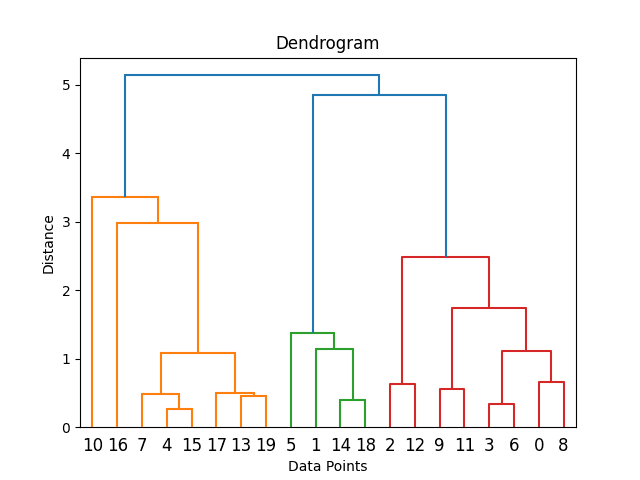
\includegraphics[width=9cm]{clustering jerarquico/figures/hierarchical-clustering-dendogram}
\end{center}

\note{
\begin{itemize}
\item <1-> Familia de algoritmos que buscan en los datos \textbf{grupos organizados jerárquicamente}. Así, a medida que se aumenten la cantidad de clusters buscados, estos se irán dividiendo o fusionando hasta alcanzar el número deseado
%\item <1-> Galaxias estructura jerarquica
\item <2-> Cada observación comienza en su propio grupo, y los pares de grupos son mezclados mientras uno sube en la jerarquía. \\
%\item <2-> Divisivas: Este es un acercamiento descendente. Todas las observaciones comienzan en un grupo, y se realizan divisiones mientras uno baja en la jerarquía.
\item <2-> Para poder decidir qué grupos deberían ser combinados o cuando un grupo debería ser dividido se requiere una \textbf{medida de disimilitud} entre conjuntos de observaciones. Esta medida es llamada \textbf{linkage}, y la libreria utilizada tiene las siguientes disponibles:
\end{itemize}
}

\end{frame}



\begin{frame}
\frametitle{Tipos de linkage}

\begin{itemize}
\item <1-> Ward
\item <2-> Complete
\item <3-> Average
\item <4-> Single
\end{itemize}

\note{
\begin{itemize}
    \item <1-> Ward: Minimiza la \textbf{suma de las diferencias al cuadrado dentro} de todos los clusters. Es un enfoque de \textbf{minimización de la varianza}.
    \item <2-> Complete: Minimiza la \textbf{distancia máxima entre observaciones} de pares de clusters.
    \item <3-> Average: Minimiza la \textbf{media de las distancias} entre todas las observaciones de pares de conglomerados.
    \item <4-> Single: Minimiza la distancia entre las observaciones \textbf{más cercanas de pares} de conglomerados.
    \item <5-> Usamos \textbf{aglomerativo} ya que parece ser el que mejores resultados da en el área de estudio \\
    %- Usamos distancia euclidiana, dado que los dominios de los datos con los cuales trabajamos son continuos \\
    \item <5-> Para \textbf{decidir sobre el linkage} a utilizar realizamos los experimentos descritos a continuacion
\end{itemize}
}

\end{frame}




\begin{frame}
\frametitle{Librería utilizada}

\begin{center}
    
\includegraphics[width=7cm]{clustering jerarquico/figures/Scikit_learn_logo_small.svg.png}
\end{center}

\vspace{0.5cm}

\center \href{https://scikit-learn.org/stable/}{https://scikit-learn.org/stable/}

\end{frame}




\begin{frame}
\frametitle{Selección de linkage}

\begin{center}
    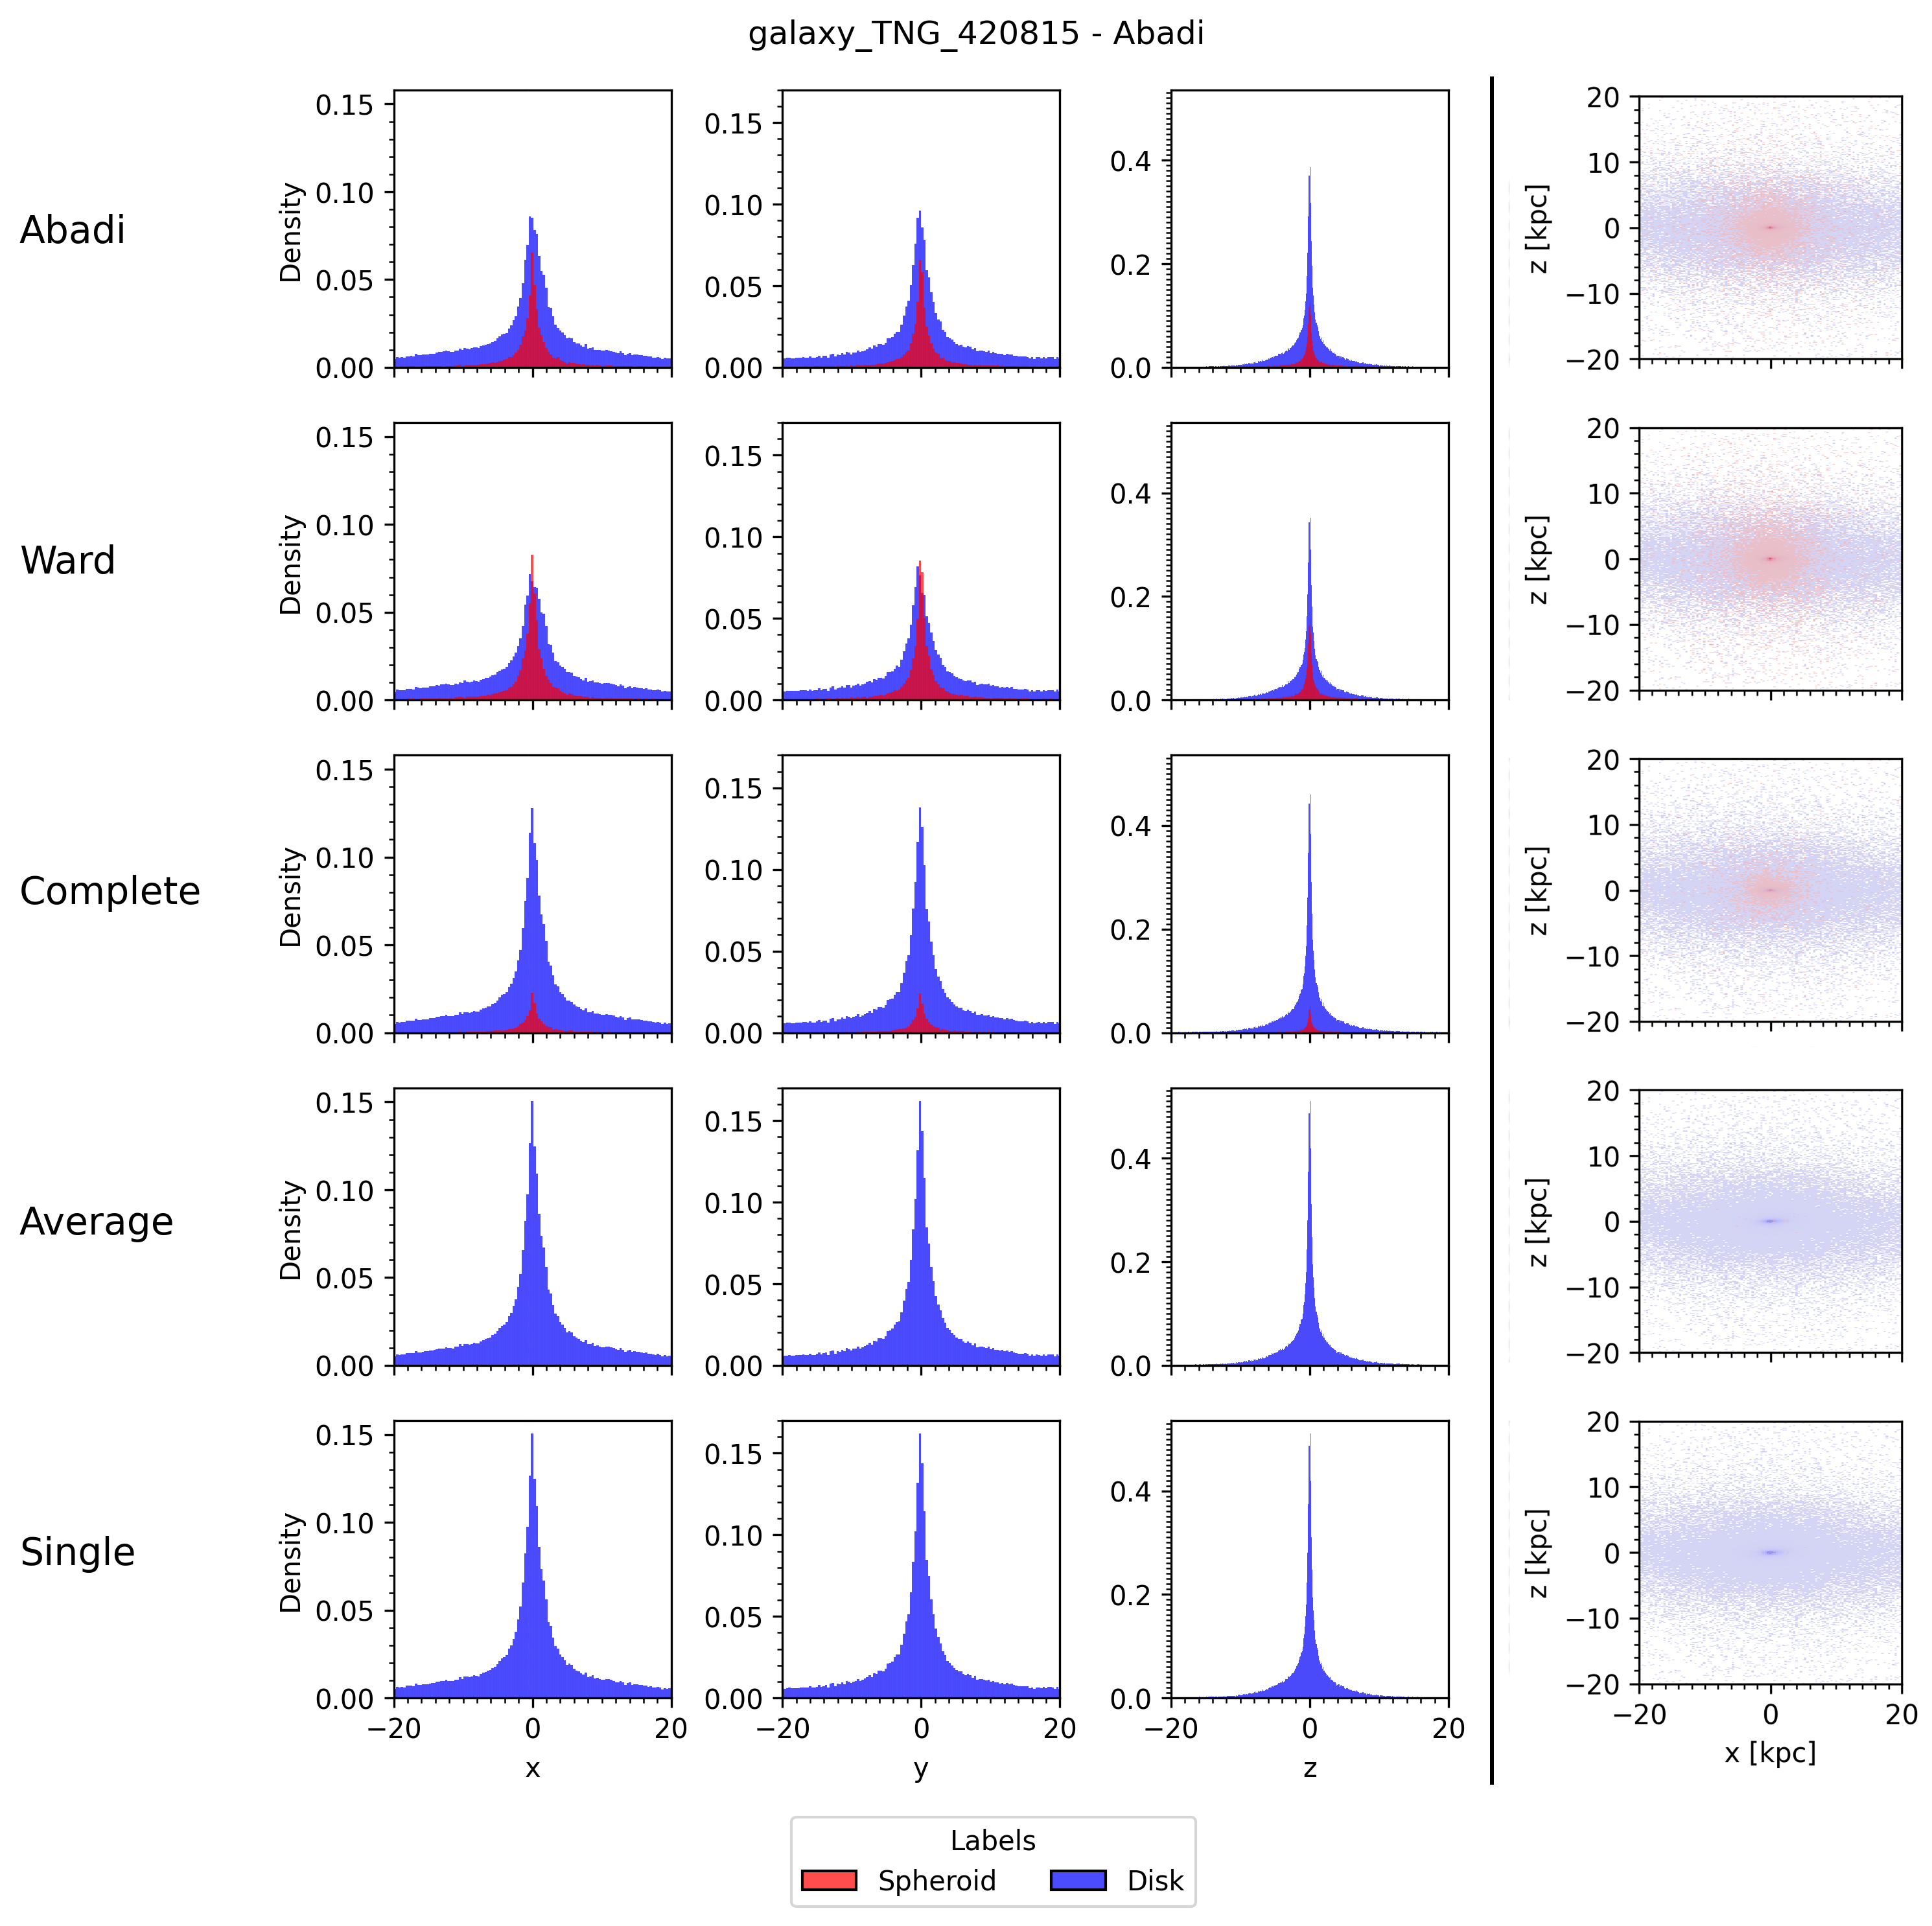
\includegraphics[width=7cm]{clustering jerarquico/figures/linkage_comparison.png}
\end{center}

\note{
- Aplicamos todos los linkages y comparamos con el método de Abadi, sobre un conjunto de 9 galaxias. \\
%- Ward da bien, puede ser por el uso de \textbf{el enfoque de las distancia intra-clusters} sea una métrica mucho más consistente e inmune al ruido en comparación al resto. \\
%- Average y Single pusieron casi todo en la \textbf{misma componente}.\\% Porque las partículas estelares de diferentes \textbf{componentes} en el espacio de circularidad están tan cercanas entre ellas que encontrar clusters se ve dificultado. \\
%- Single el cual hace uso de la distancia mínima inter-clusters, basta con tener un solo punto alejado del resto de nuestros datos para que éste sea identificado como un único cluster. \\
%- Average: su tarea se ve perjudicada por el alto solapamiento de los clusters \\
%- Complete: si bien da algunos resultados similares a Abadi, es \textbf{inestable} y no logra resultados con la consistencia que logra Ward en el apendice \\
}

\end{frame}

%capaz mostrar lo cerca que estan las particulas en cada feature?


\begin{frame}
\frametitle{Abadi: Detección de 2 componentes}

\begin{center}
    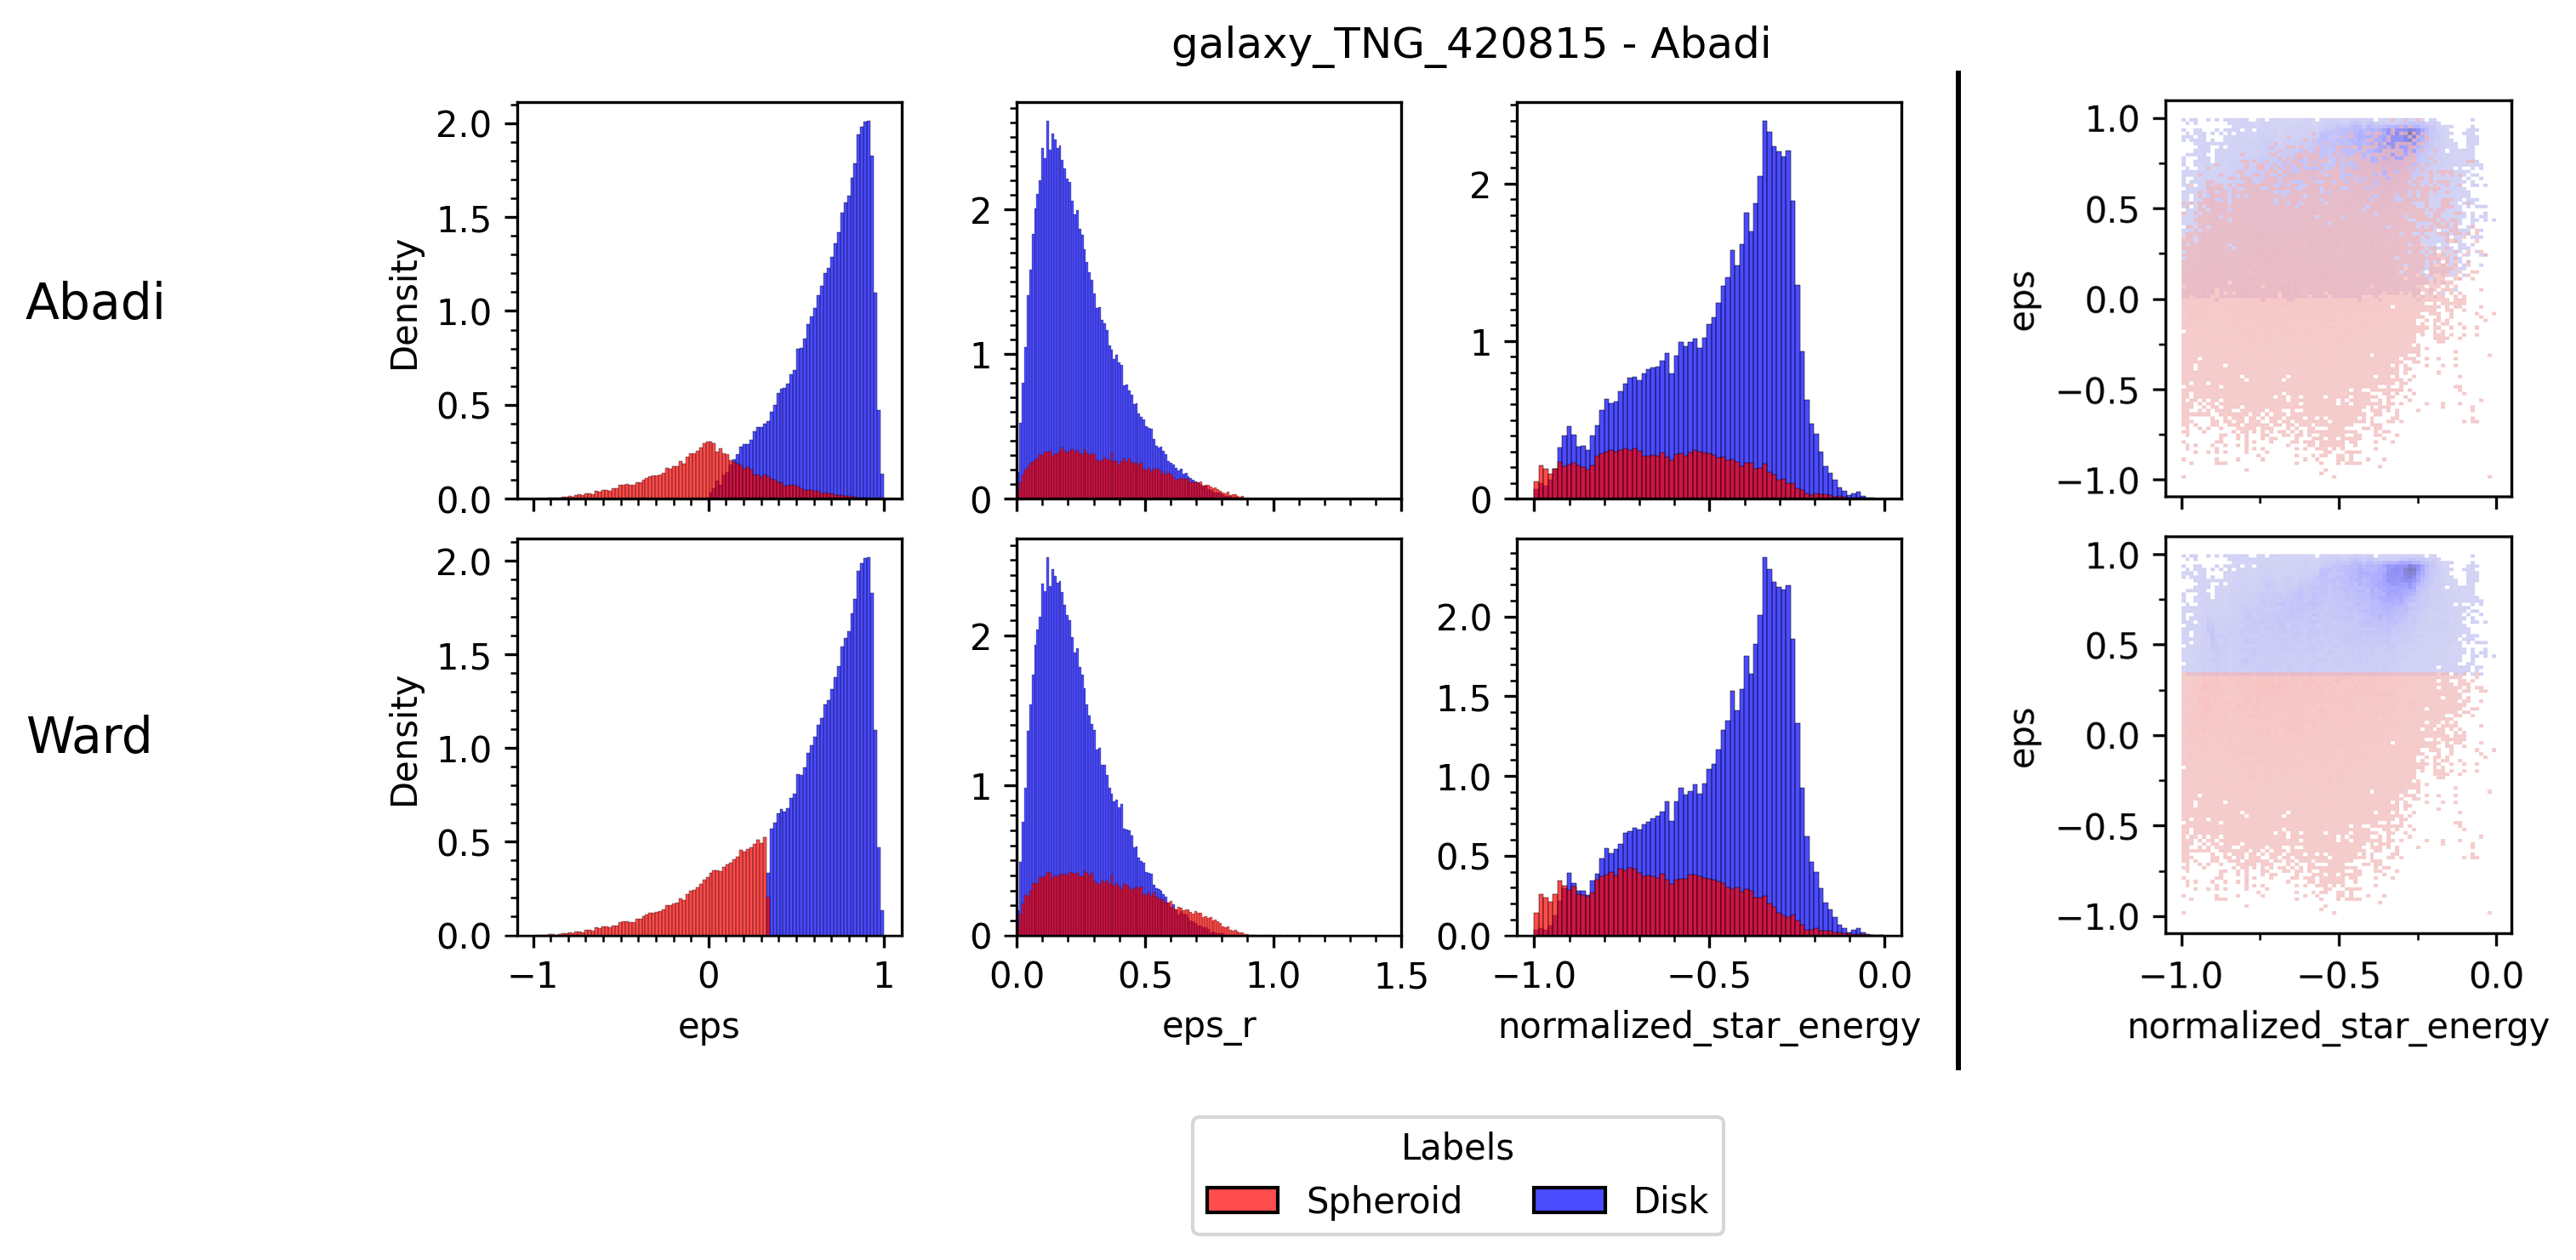
\includegraphics[width=8cm]{clustering jerarquico/figures/galaxy_TNG_420815 - abadi - base - circ histogram and scatterplot.png}
    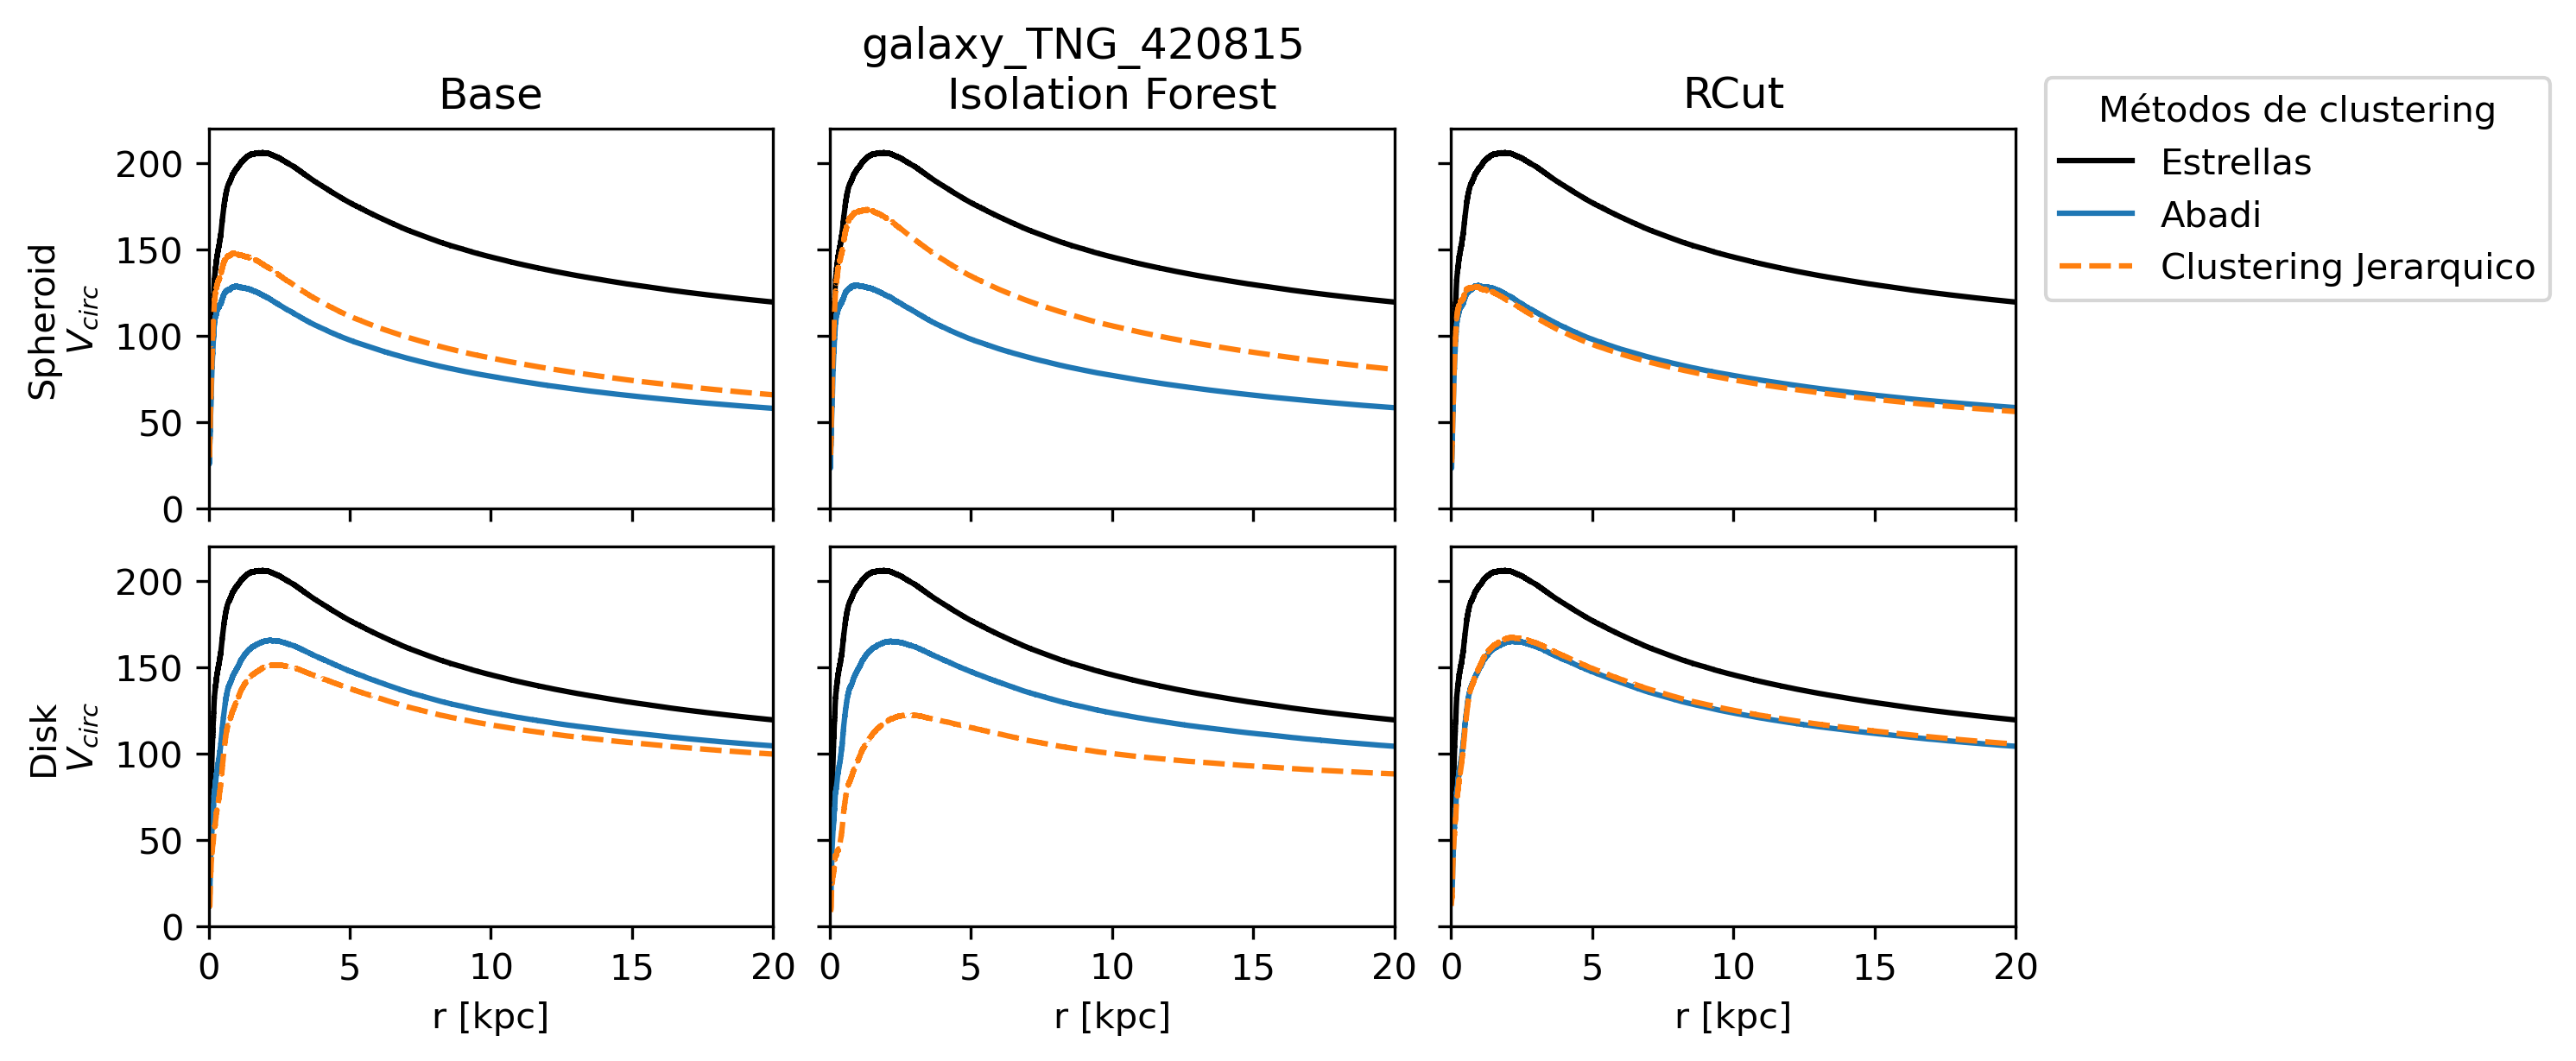
\includegraphics[width=8cm]{clustering jerarquico/figures/galaxy_TNG_420815 - Abadi - circ_velocity.png}
\end{center}

\note{
%- parametro vs feature \\
- recordamos que se usan las \textbf{mismas features que Abadi}, buscando 2 clusters \\
- \textbf{corte en vertical} feo por falta de heuristica, es el \textbf{mejor resultado} al cual se puede aspirar\\
- Esta situación hace que haya una \textbf{sobreestimacion del esferoide} como se ve en los perfiles de velocidad \\
}

\end{frame}




% presicion y recall
%bastante bien (penultimo parrafo de seccion 3.2
% los resultados parecen converger a los de abadi
%podria ser mejor (ultimo parrafo seccion 3.2)



%\begin{frame}
%\frametitle{Abadi: Eliminación de outliers}

%\begin{center}
%    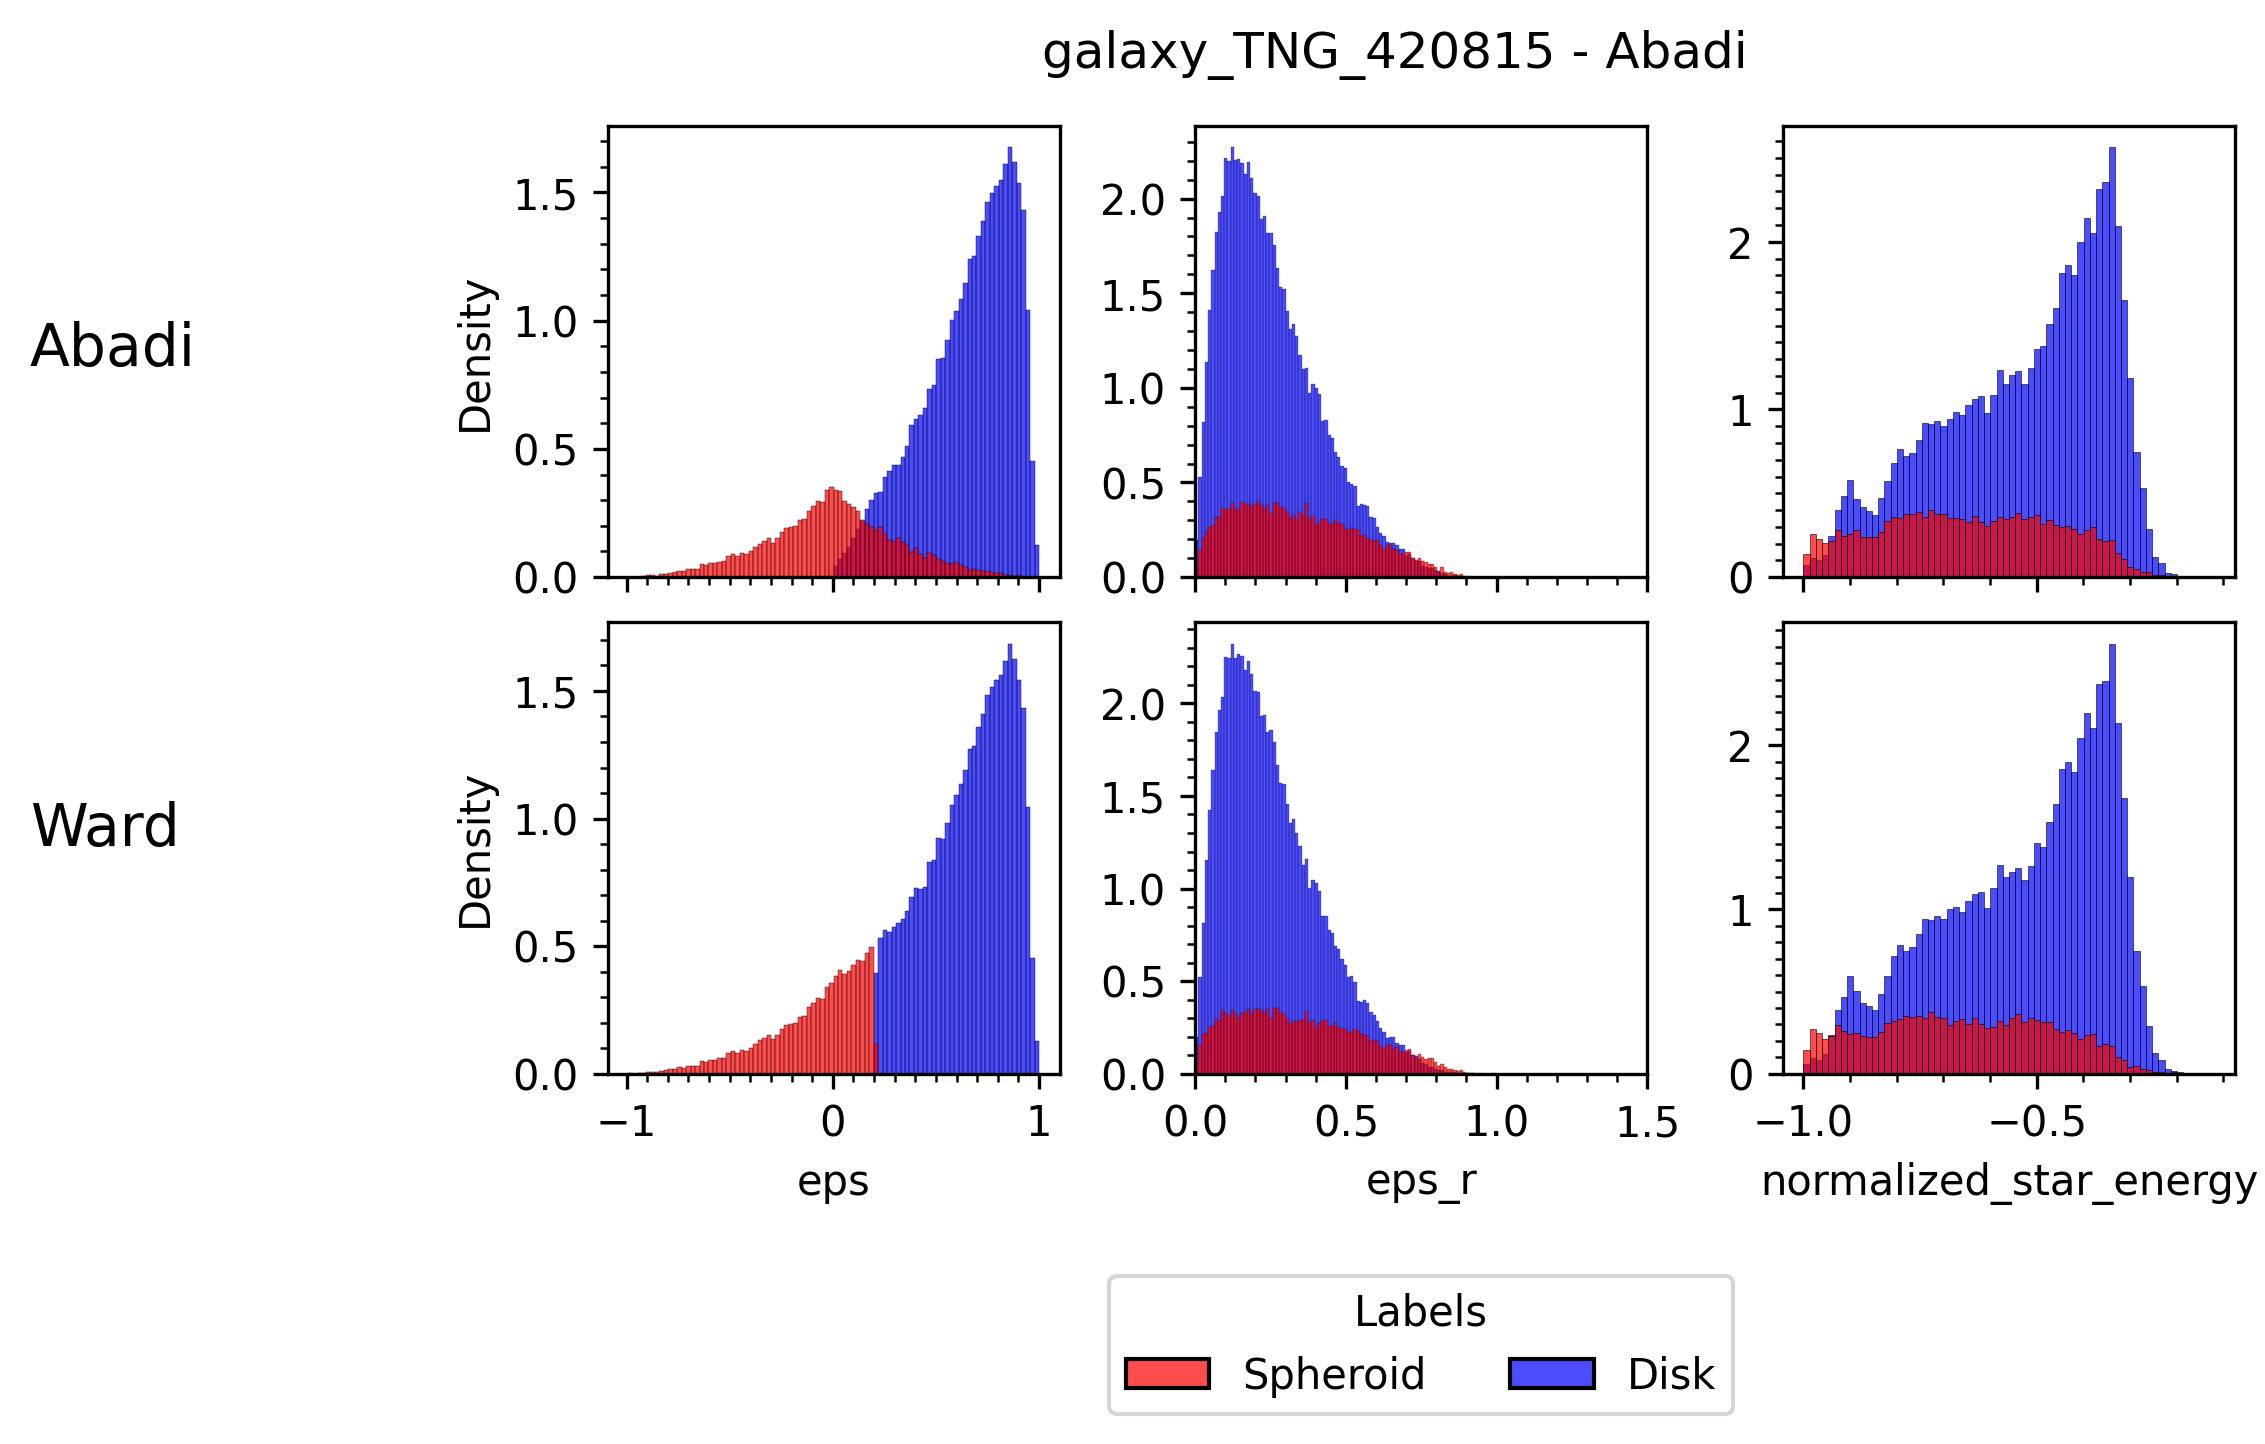
\includegraphics[width=12cm]{clustering jerarquico/figures/galaxy_TNG_420815 - abadi - rcut - circ histogram.png}
%\end{center}

%\note{
%Esto que vemos es RCut
%}

%\end{frame}




\begin{frame}
\frametitle{Abadi: Eliminación de outliers}

\begin{columns}
\column{0.5\textwidth}
\begin{center}
    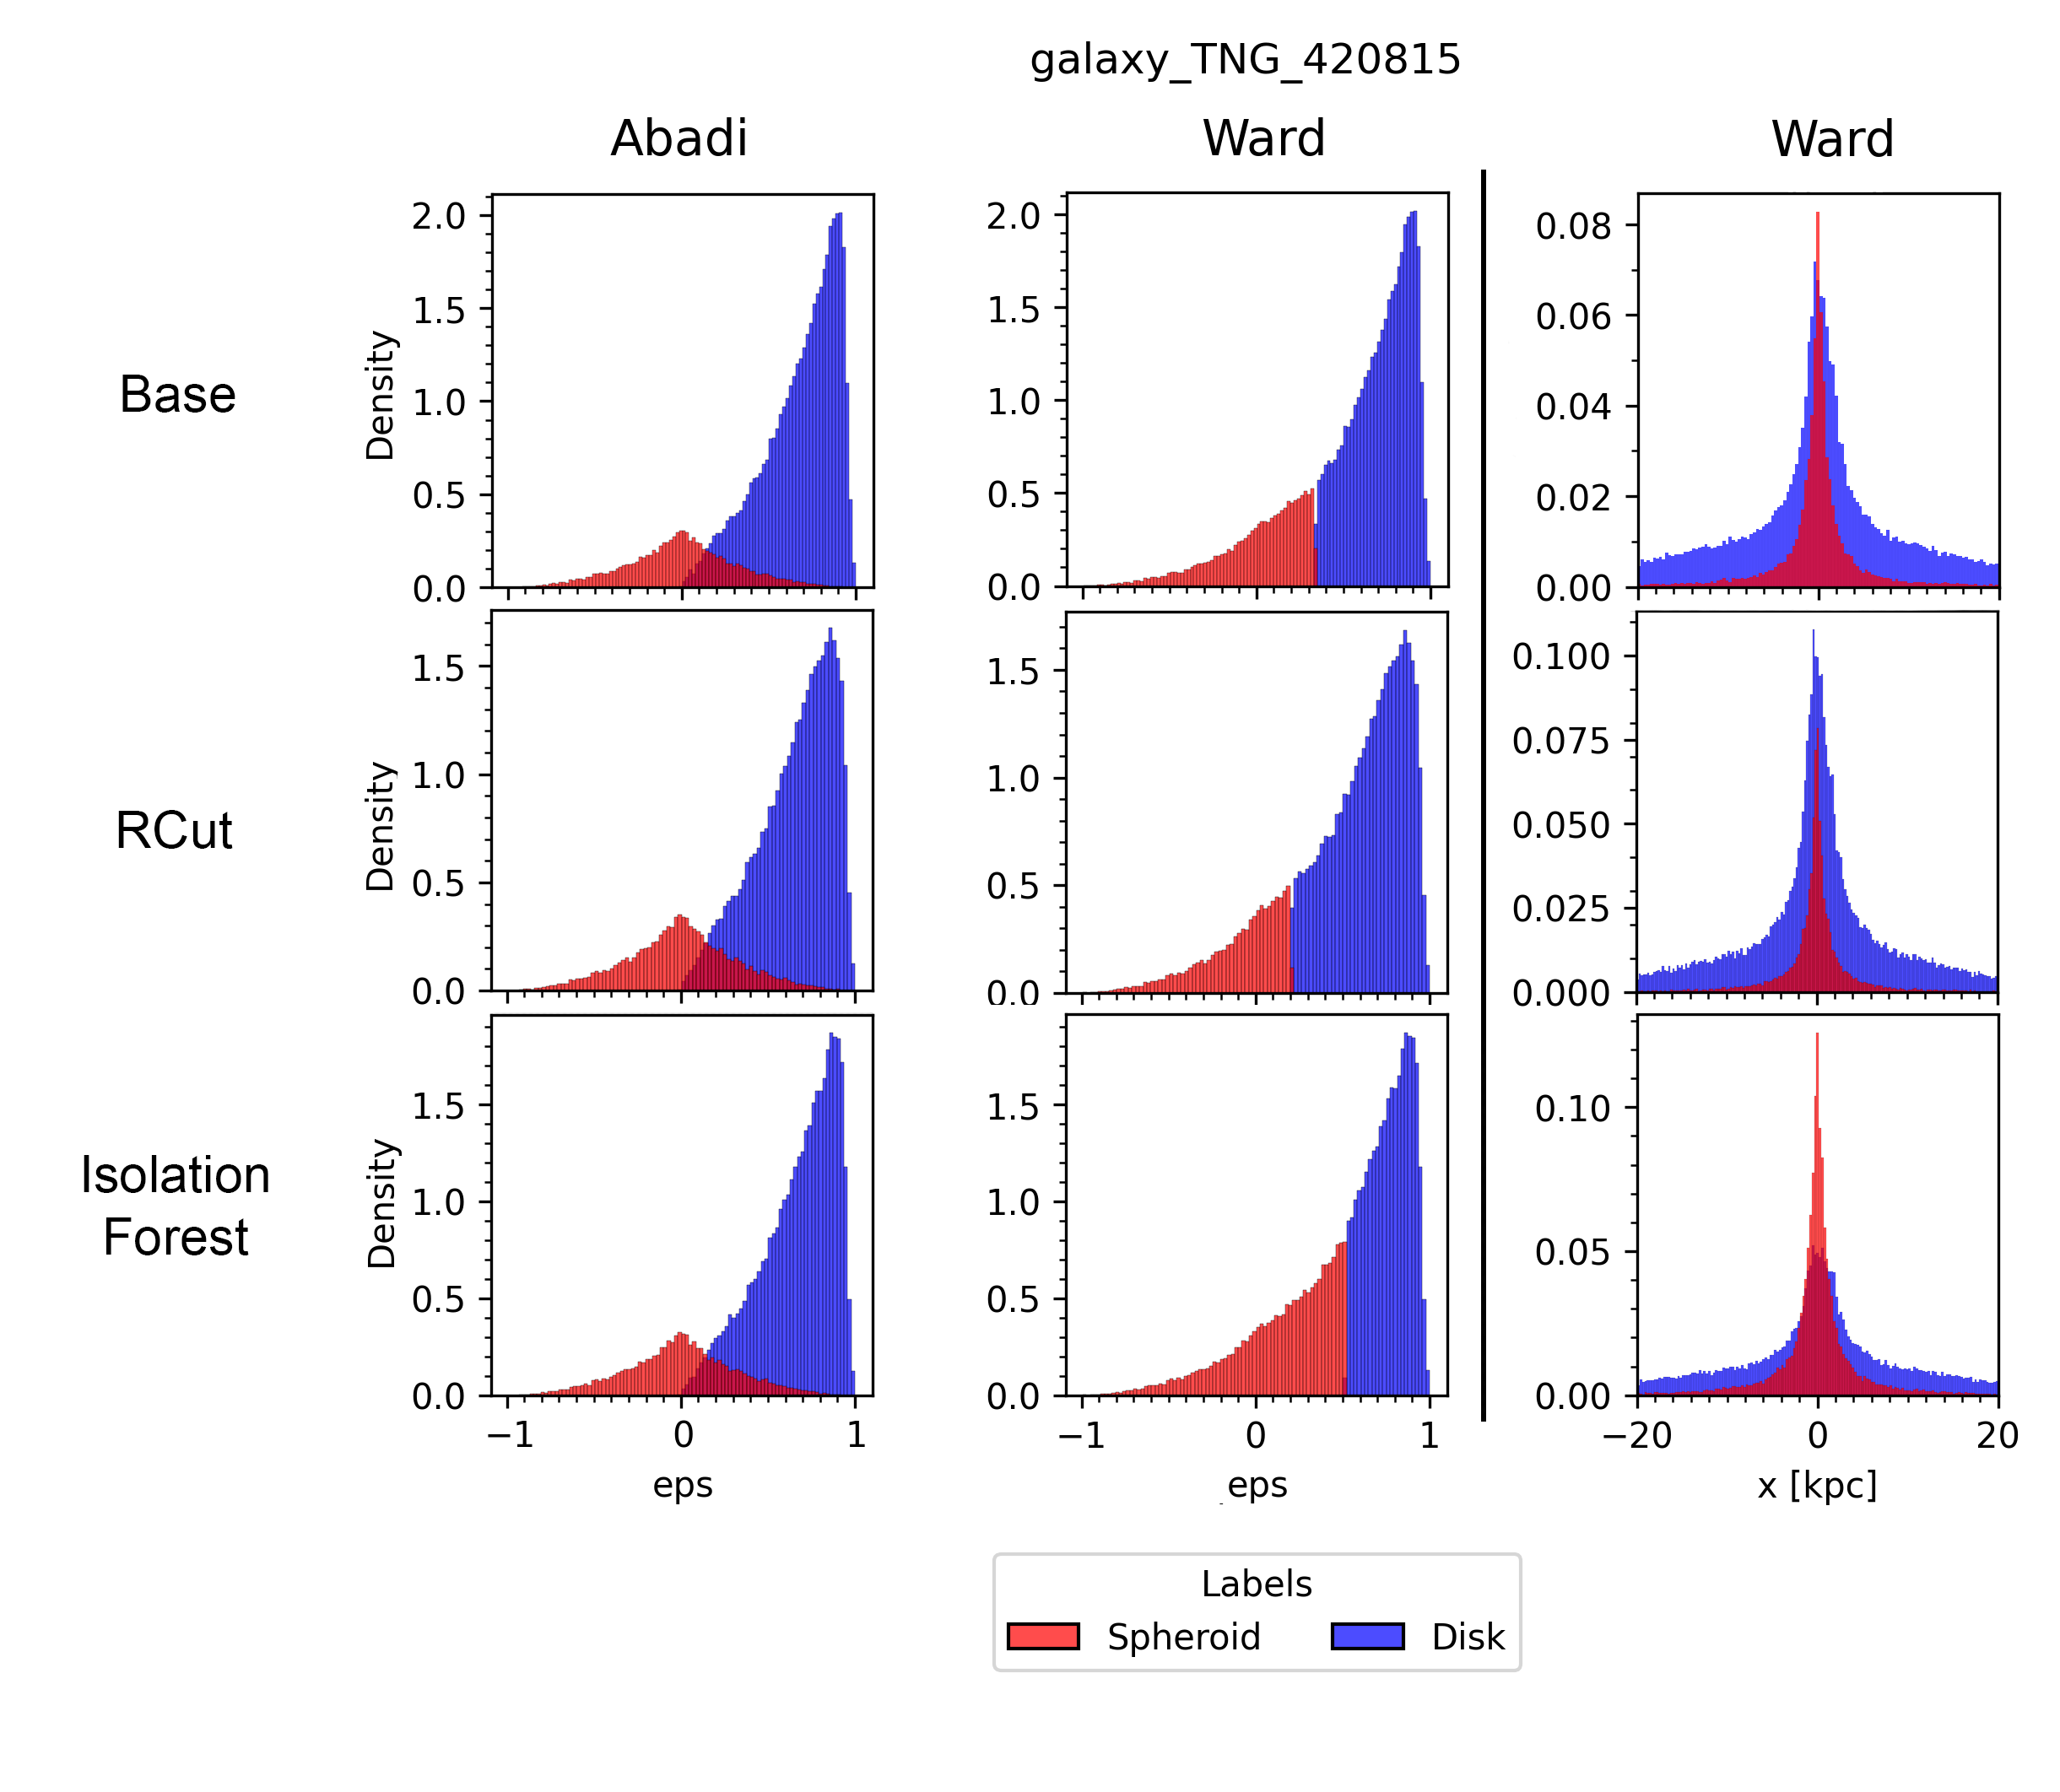
\includegraphics[width=6cm]{clustering jerarquico/figures/galaxy_TNG_420815 - abadi - base vs rcut vs isolation forest.png}
\end{center}
\column{0.5\textwidth}
\begin{center}
    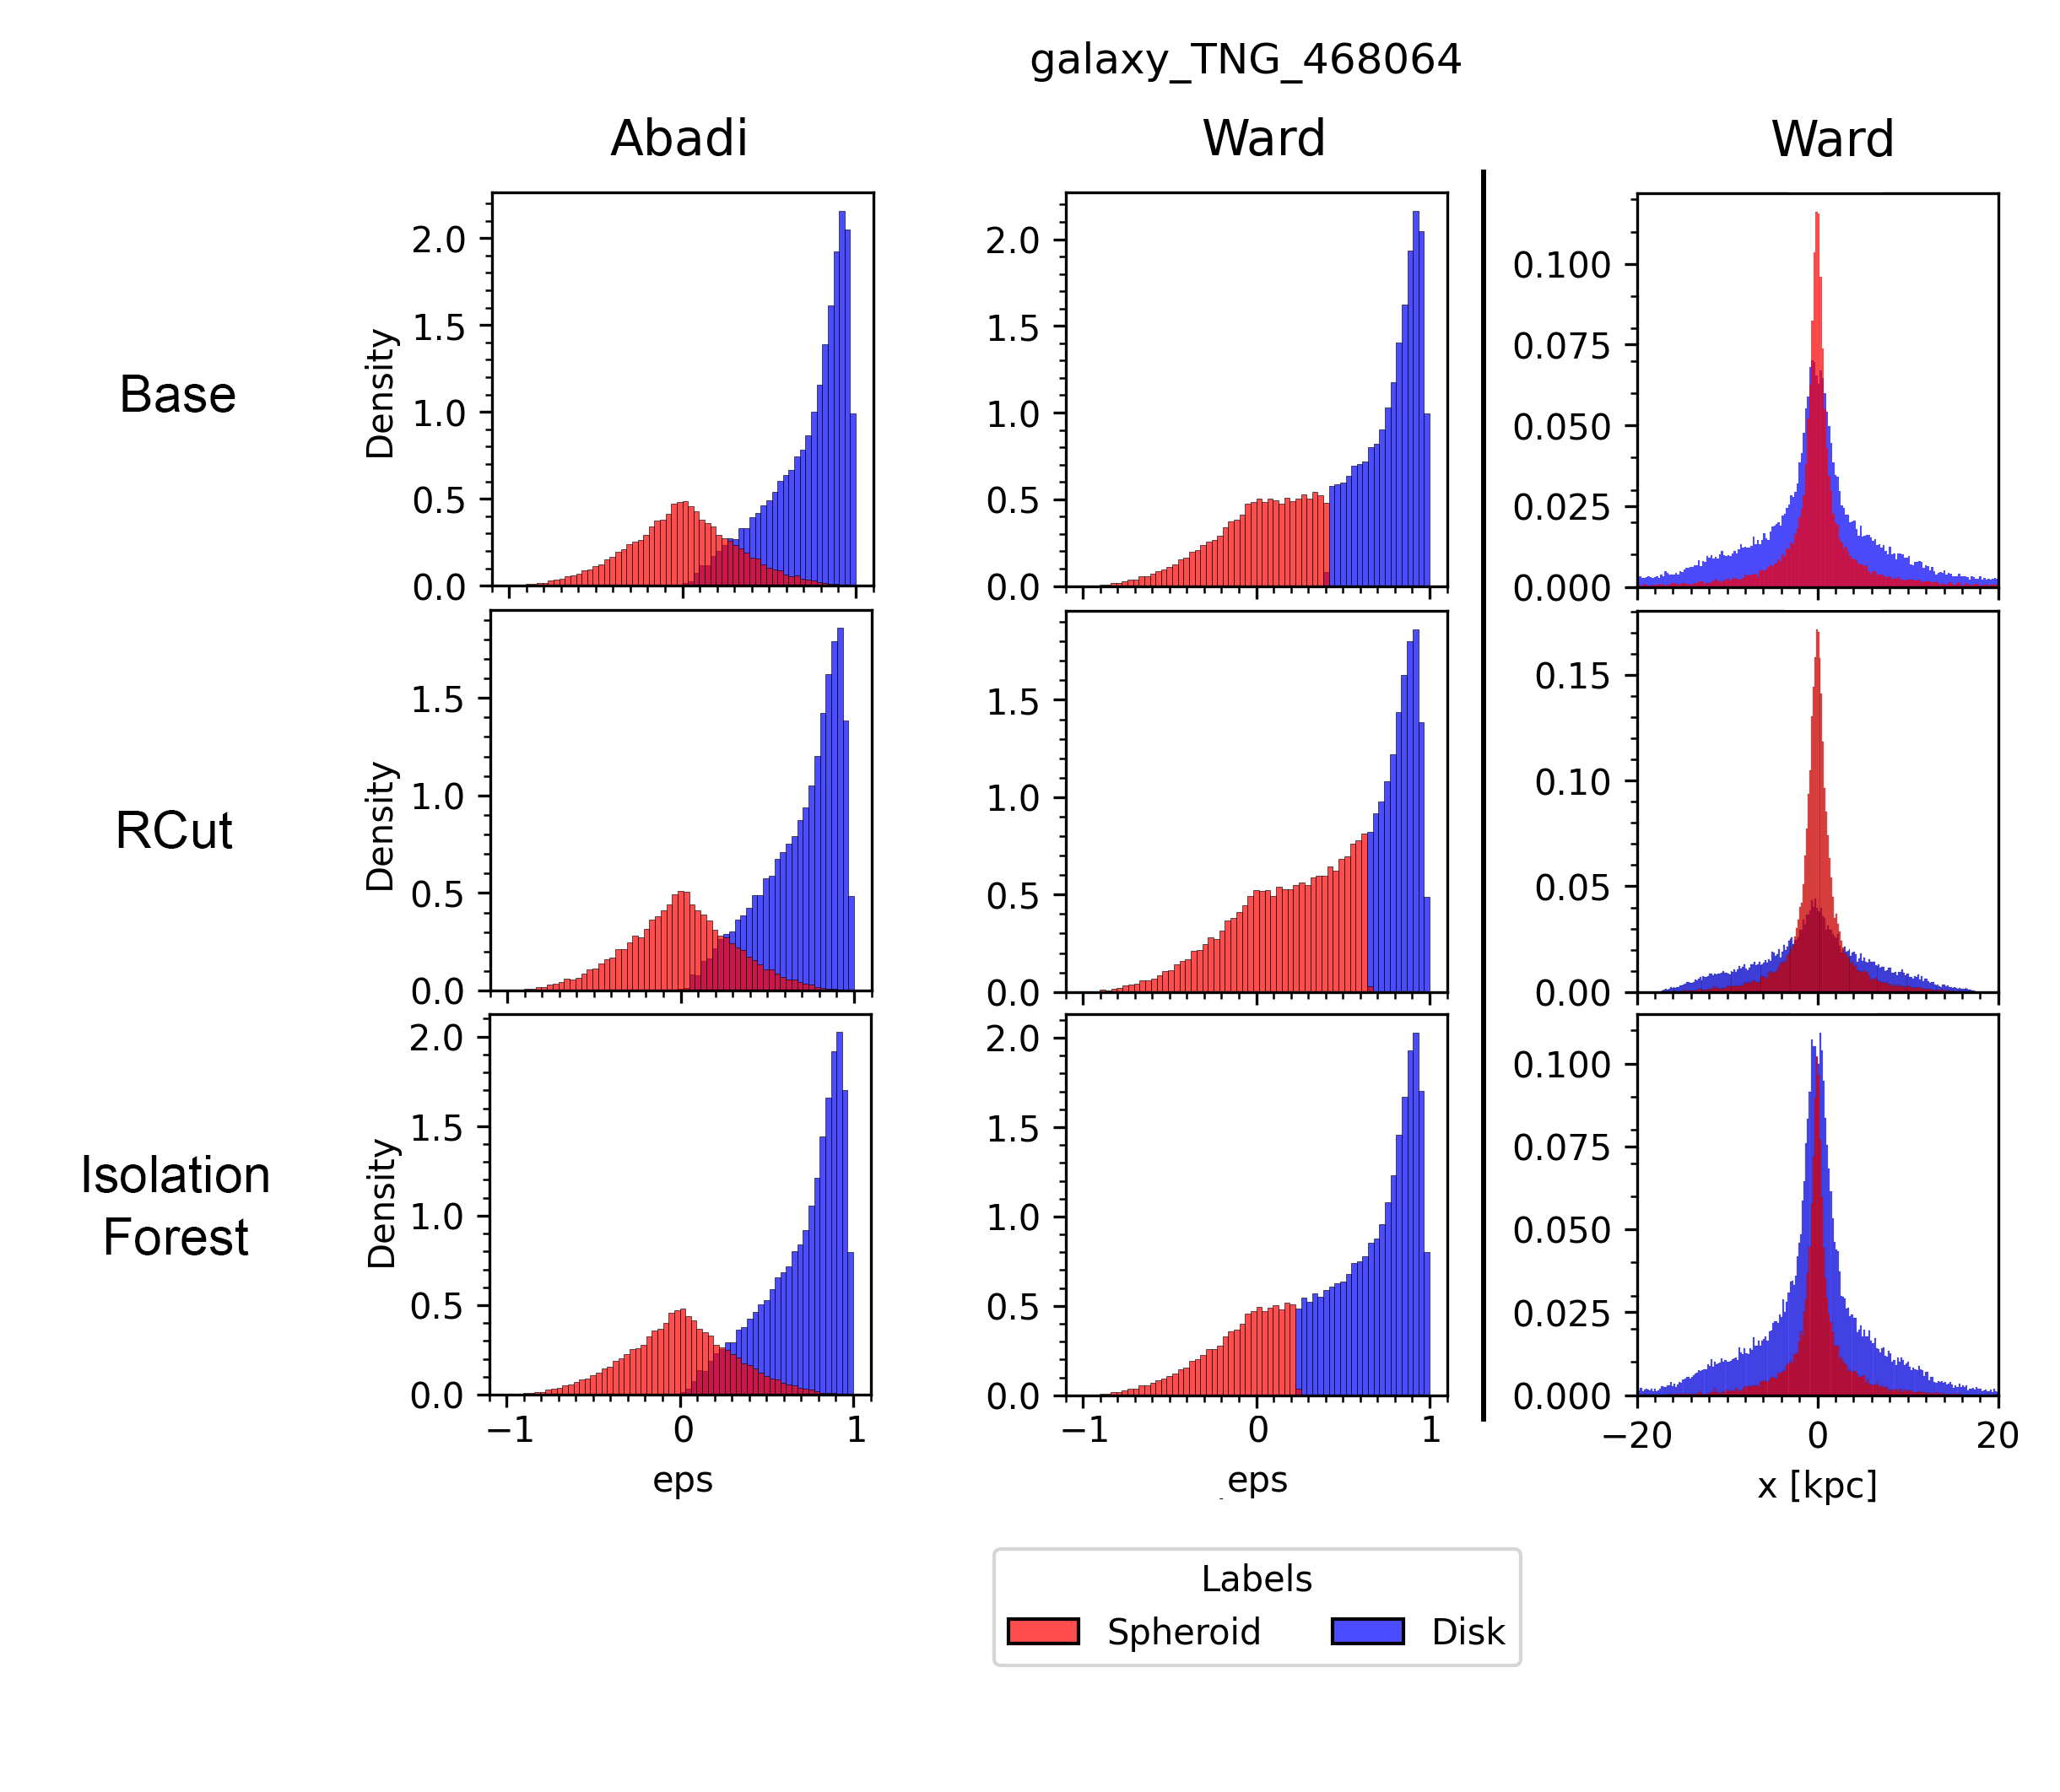
\includegraphics[width=6cm]{clustering jerarquico/figures/galaxy_TNG_468064 - abadi - base vs rcut vs isolation forest.png}
\end{center}
\end{columns}

\note{
%- cambio por que ahora el pico de densidad del esferoide bajo, entonces al minimizar la varianza cambio la linea de corte \\
%- hipotesis erronea, no podemos concluir si ayuda o no \\
- \textbf{no podemos concluir} que ayuda ni que no, para rcut ni para isolation forest \\
}

\end{frame}


\begin{frame}
\frametitle{Abadi: Eliminación de outliers}

\begin{columns}
\column{0.5\textwidth}
\begin{center}
    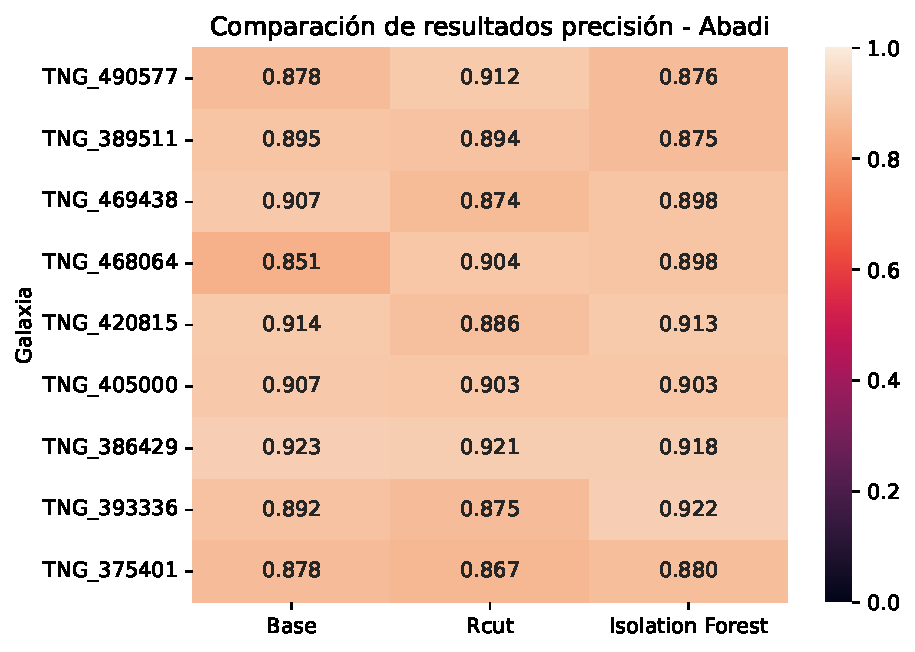
\includegraphics[width=6cm]{clustering jerarquico/figures/precision - abadi.pdf}
\end{center}
\column{0.5\textwidth}
\begin{center}
    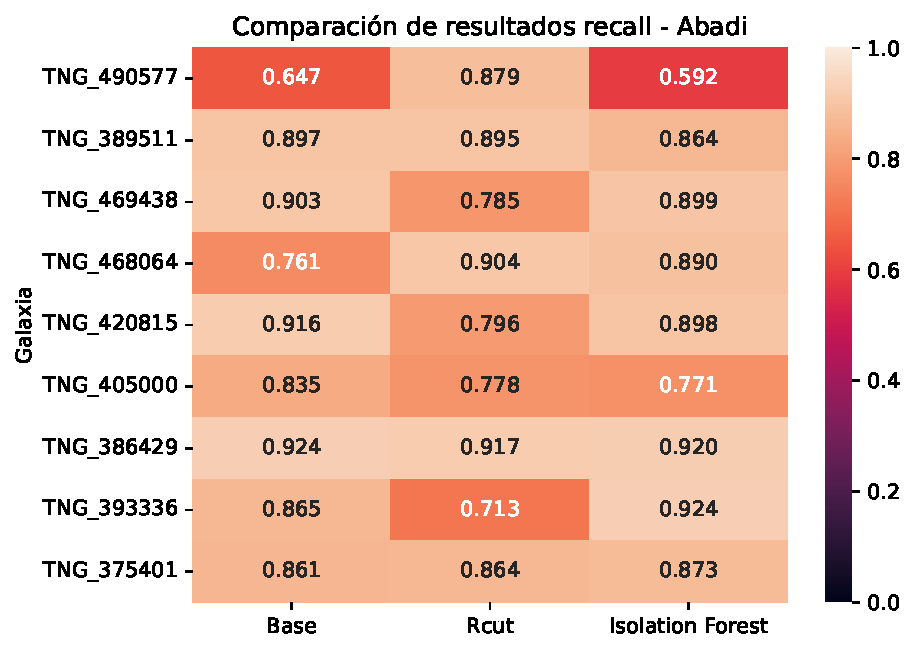
\includegraphics[width=6cm]{clustering jerarquico/figures/recall - abadi.pdf}
\end{center}
\end{columns}

\note{
- aunque en lineas generales parece dar \textbf{bien} le falta la sutileza de la \textbf{interpretacion fisica} que le da abadi a los valores \\
%- no son resultados concluyentes para decir si es bueno o no sacar outliers \\
- cj es \textbf{mas caro computacionalmente} que abadi ($O(n^2)$), incluso si da mejor no nos sirve como alternativa del dia a dia
}

\end{frame}


% cj es mas caro que abadi, incluso si da mejor no nos sirve como alternativa del dia a dia
% Como nota final, podemos concluir que el \gls{HC} se comporta, como mucho, de forma similar a Abadi al buscar 2 clusters, pero como éste es más caro en memoria y computacionalmente (ya que calcula una matriz de distancia, por lo que estamos hablando de magnitudes de $O(n^2)$ para ambos), al final del día el algoritmo de Abadi sigue siendo la mejor alternativa.



\begin{frame}
\frametitle{AGMM: Detección de $=>$2 componentes}

\begin{center}
    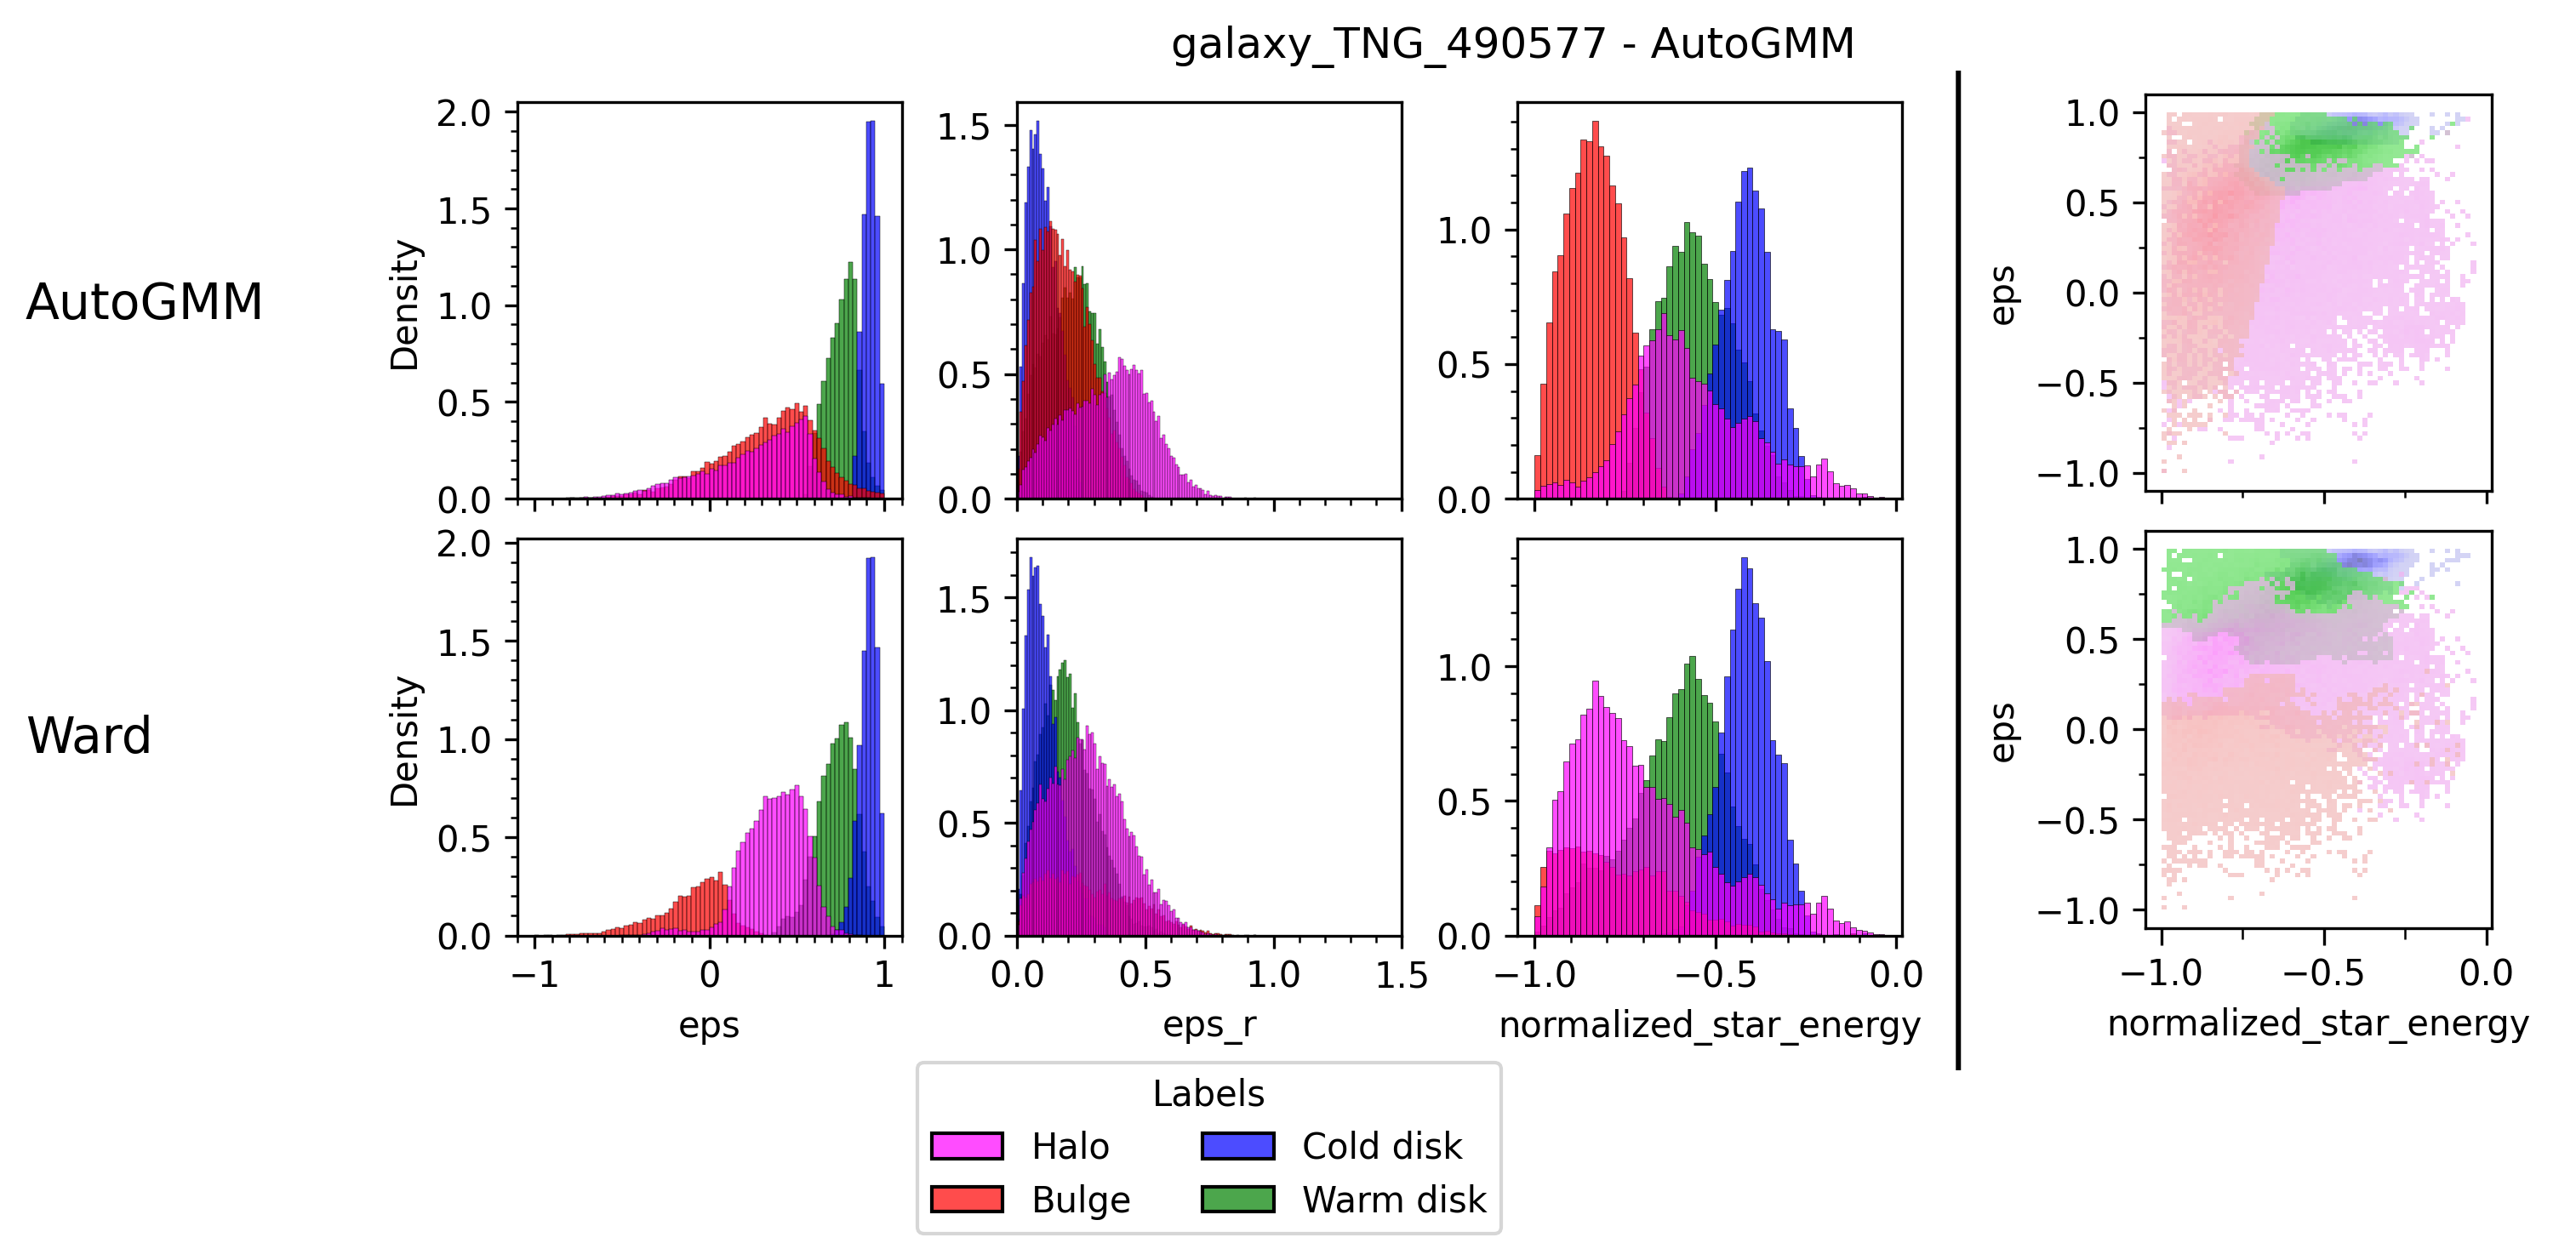
\includegraphics[width=12cm]{clustering jerarquico/figures/AGMM - galaxy_TNG_490577 - circ histogram.png}
\end{center}

\note{
%- Si nos dio mal los linkages antes seria raro que nos de bien ahora, por eso partimos directamente usando Ward \\
%- Idea jerarquica de las componentes. Al comparar contra Abadi antes, esperariamos que ahora, al buscar mas componentes, encontremos el \textbf{Disco fino y grueso dentro de lo que era el Disco}. No es un problema para el Disco, pero lo es con el Esferoide \\
%- Explicar porque se \textbf{solapa halo y bulge en AGMM, pero no en HC}: Como \textbf{Esferoide} es soportado por dispercion de velocidades, sus \textbf{particulas tienen gran variacion en eps}. Esto tambien es verdad para sus \textbf{subcomponentes}, Halo y Bulge, por lo que se ven solapadas en AGMM. \\
- \textbf{Halo y Bulge se ven separados en eps en lugar de solapados}\\
- Como el linkage \textbf{Ward} busca \textbf{minimizar la varianza de cada cluster}, esto se traduce en buscar que los \textbf{clusters estén lo más separados entre ellos}, lo cual va en directa contraposición con la \textbf{naturaleza de las componentes mencionadas} (incluso si esta bien para clusterizacion en general)
}



\end{frame}

\iflong
\begin{frame}
\frametitle{AGMM: Detección de $=>$2 componentes}

\begin{center}
    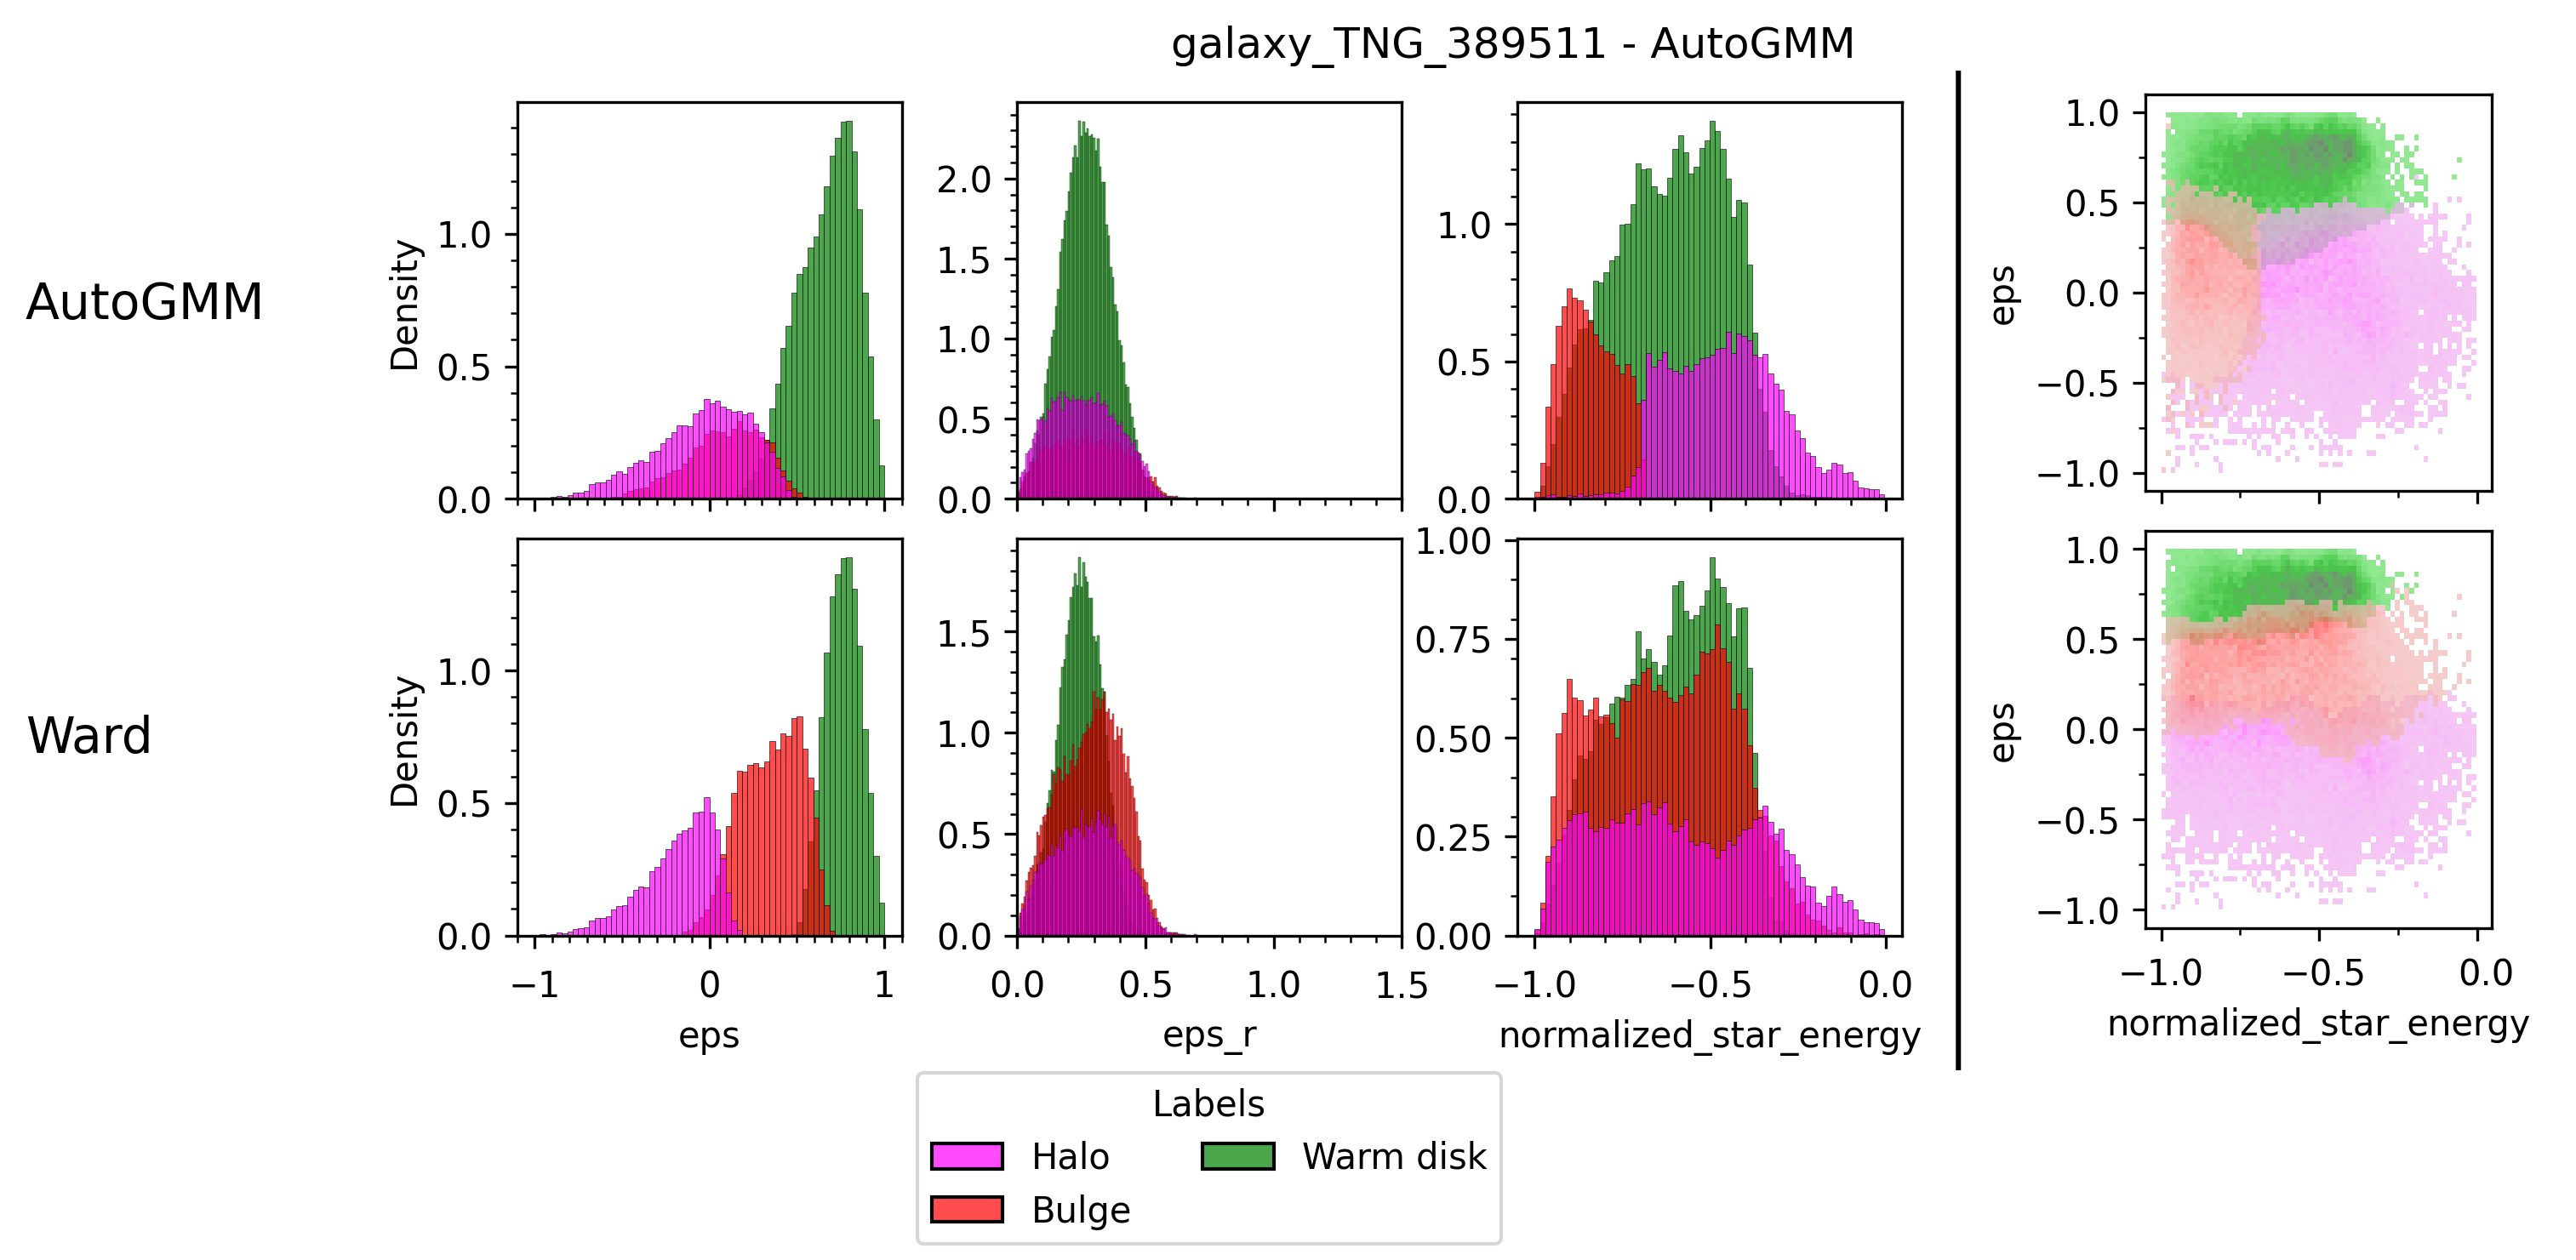
\includegraphics[width=12cm]{clustering jerarquico/figures/AGMM - galaxy_TNG_389511 - circ histogram.png}
\end{center}

\note{
- \textbf{$eps$ no es una buena feature para identificar Halo y Bulge}. La \textbf{siguiente mejor es $normalized\_star\_energy$} segun el orden de relevancia en el area. Y podemos confirmar su importancia al mirar como se dividen estas en AGMM. Pero el Warm disk solapa ahi y le complica a Ward usar la feature como corresponde para identificar componentes. Corte unidimensional en el scatterplot.\\
%- Como las componentes del Disco son soportadas por rotación, esto significa que predomina el movimiento ordenado, por lo que ambos discos tienen sus componentes mas acotadas en eps y son mas faciles de identificar por CJ (diapo anterior). \\
}

\end{frame}
\fi

\begin{frame}
\frametitle{AGMM: Detección de $=>$2 componentes}

\begin{columns}
\column{0.5\textwidth}
\begin{center}
    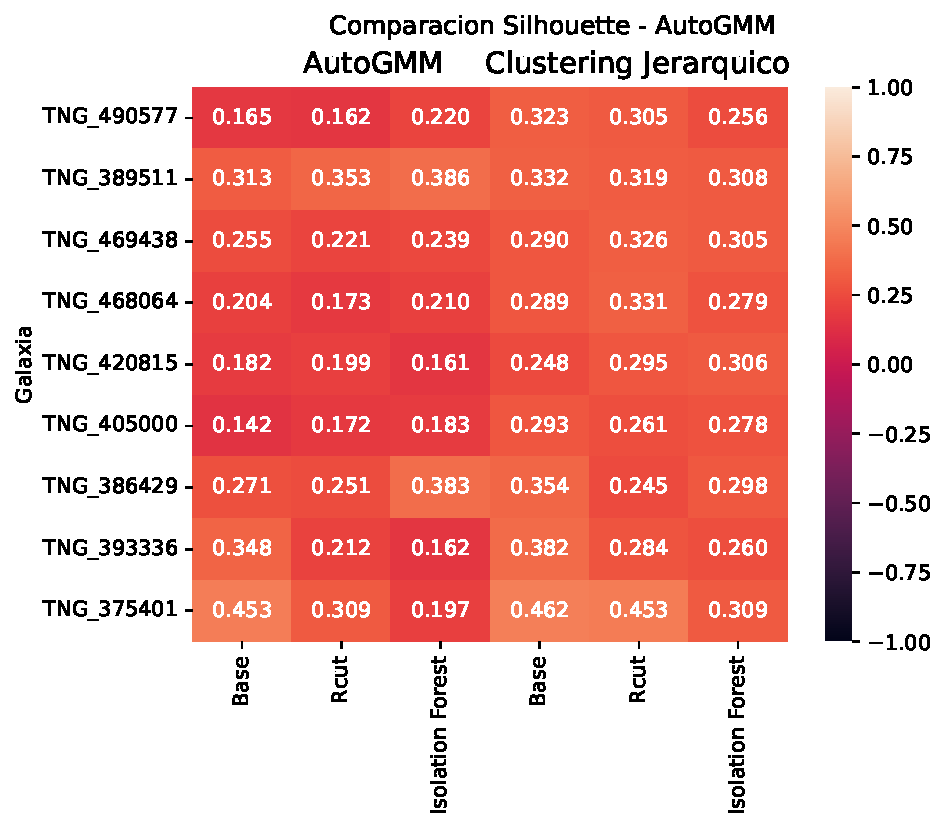
\includegraphics[width=6cm]{clustering jerarquico/figures/silhouette - agmm.pdf}
\end{center}
\column{0.5\textwidth}
\begin{center}
    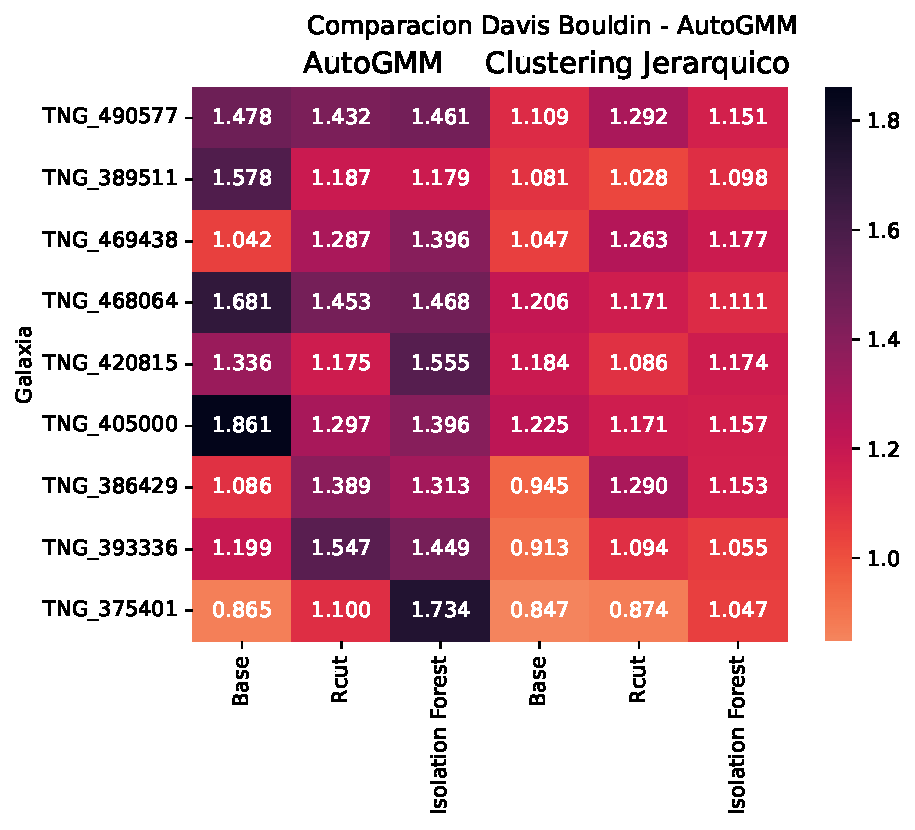
\includegraphics[width=6cm]{clustering jerarquico/figures/davis bouldin - agmm.pdf}
\end{center}
\end{columns}

\note{
- Las metricas internas dicen que ward da mejor que agmm, pero \textbf{esta mal} \\
- Distinción entre lo que es \textbf{más correcto} a la hora de \textbf{buscar clusters abstractos} contra buscar componentes de una galaxia \\
- Estas métricas son calculadas a partir del \textbf{concepto ideal abstracto de cluster}, el cual se basa en que éstos sean compactos, separados espacialmente están entre ellos, y que exista ``continuidad'' en cada uno. \\
}

\end{frame}


\iflong
\begin{frame}
\frametitle{AGMM: Detección de $=>$2 componentes}

\begin{columns}
\column{0.5\textwidth}
\begin{center}
    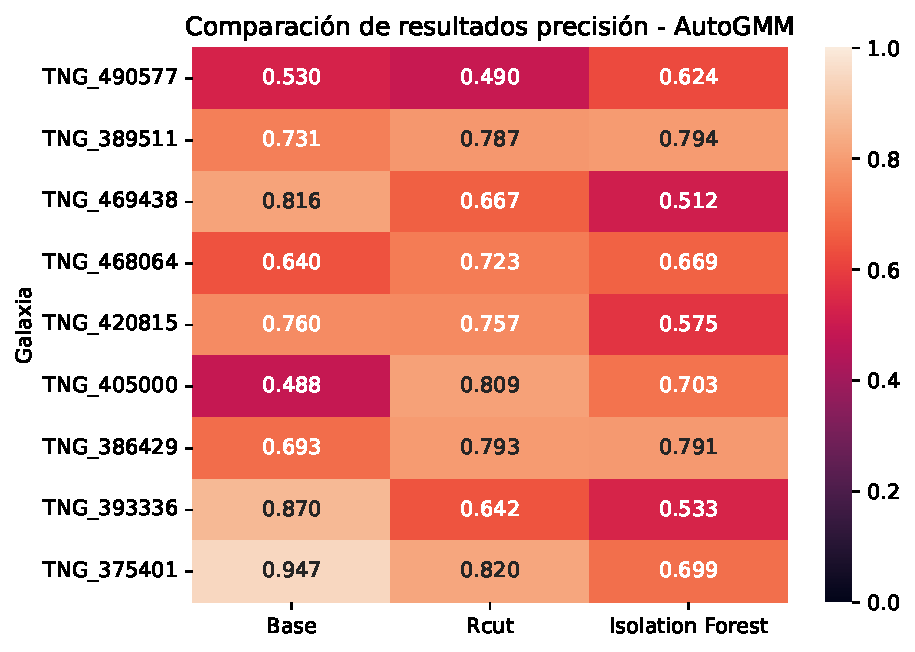
\includegraphics[width=6cm]{clustering jerarquico/figures/precision - agmm.pdf}
\end{center}
\column{0.5\textwidth}
\begin{center}
    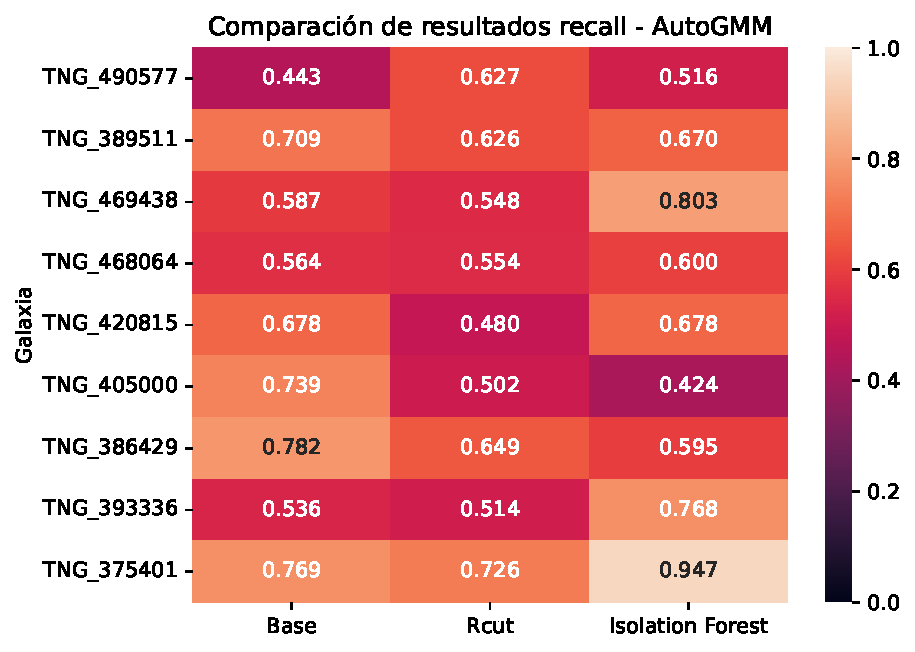
\includegraphics[width=6cm]{clustering jerarquico/figures/recall - agmm.pdf}
\end{center}
\end{columns}

\note{
- presicion y recall promedio dan mas de 0.5 pero no mucho mas, por lo que no son muy buenas \\
%- las soluciones del método jerárquico con más clusters son particiones de las soluciones con menos clusters, por lo cual solo pueden aumentar el error al aumentar la cantidad de clusters a buscar (mas clusters a buscar va a empeorar el error)
}

\end{frame}
\fi



\begin{frame}
\frametitle{AGMM: Eliminación de outliers}

\begin{center}
    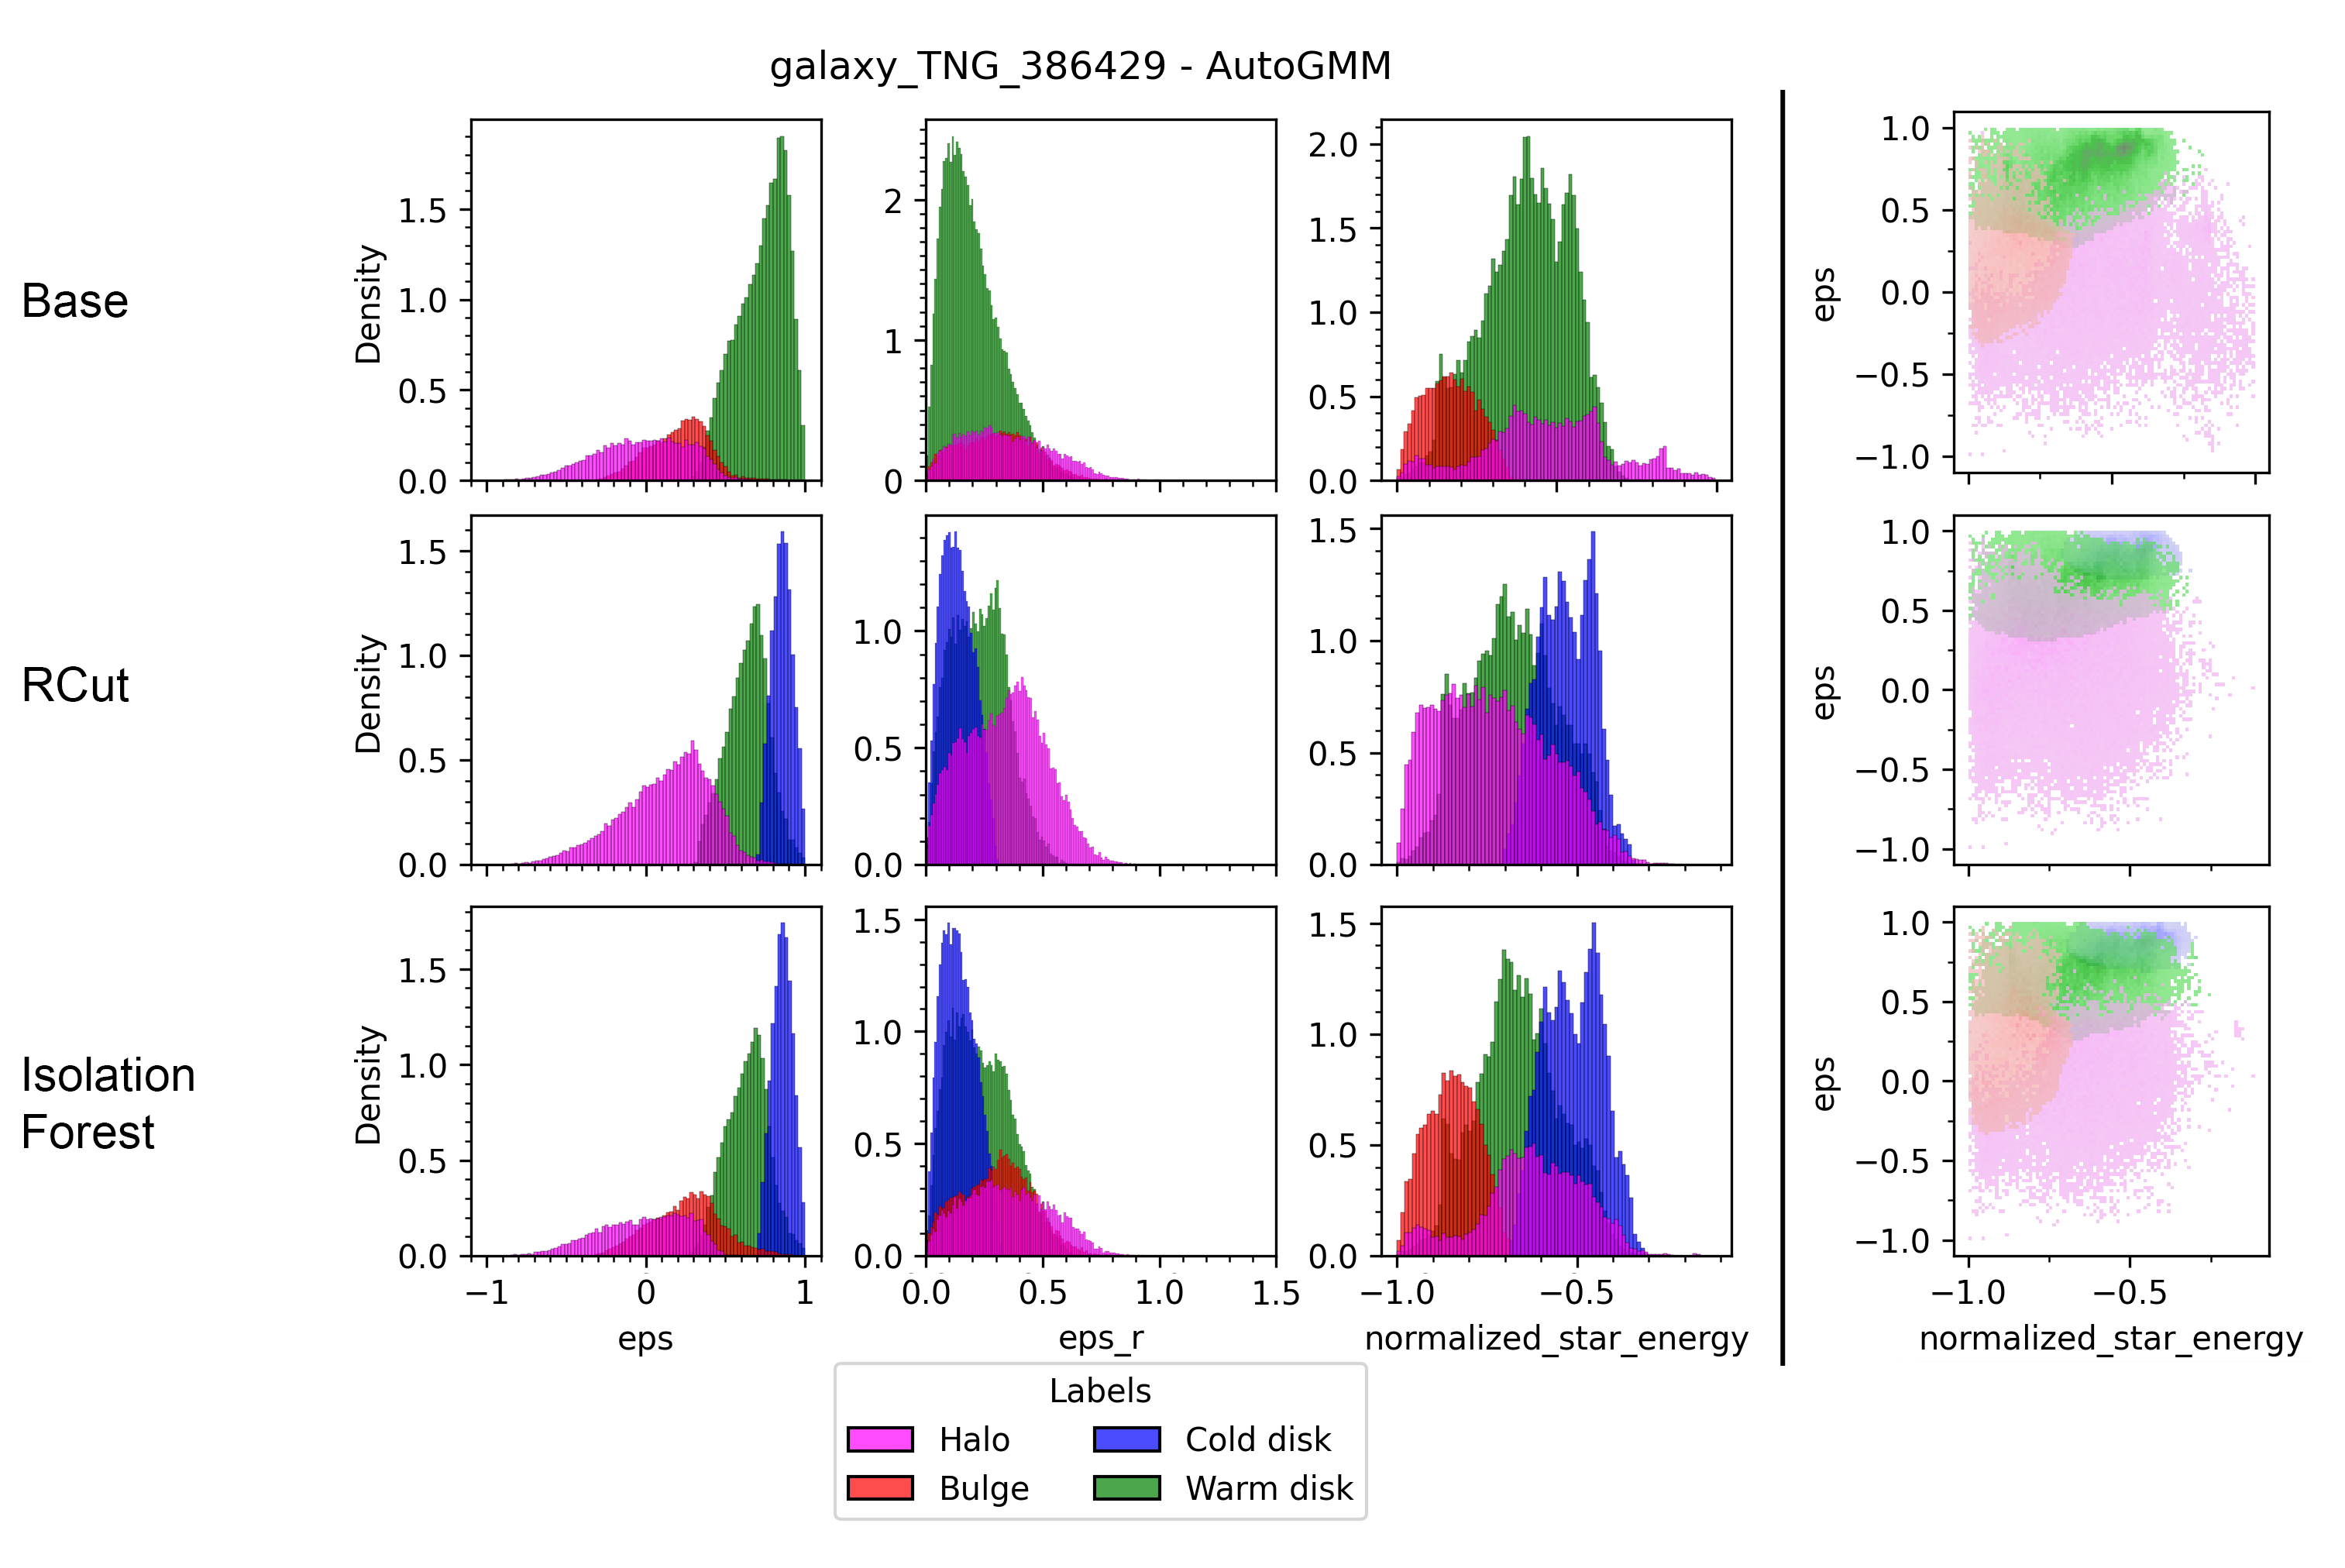
\includegraphics[width=12cm]{clustering jerarquico/figures/AGMM - different components found.png}
\end{center}

\note{
- remover outliers te puede cambiar la \textbf{cantidad de clusters} encontrados por como funciona agmm, lo cual dificulta la comparacion \\
}

\end{frame}


\begin{frame}
\frametitle{AGMM: Eliminación de outliers}
% - igualmente, con los datos que tenemos no podemos decir que sirva
\begin{center}
    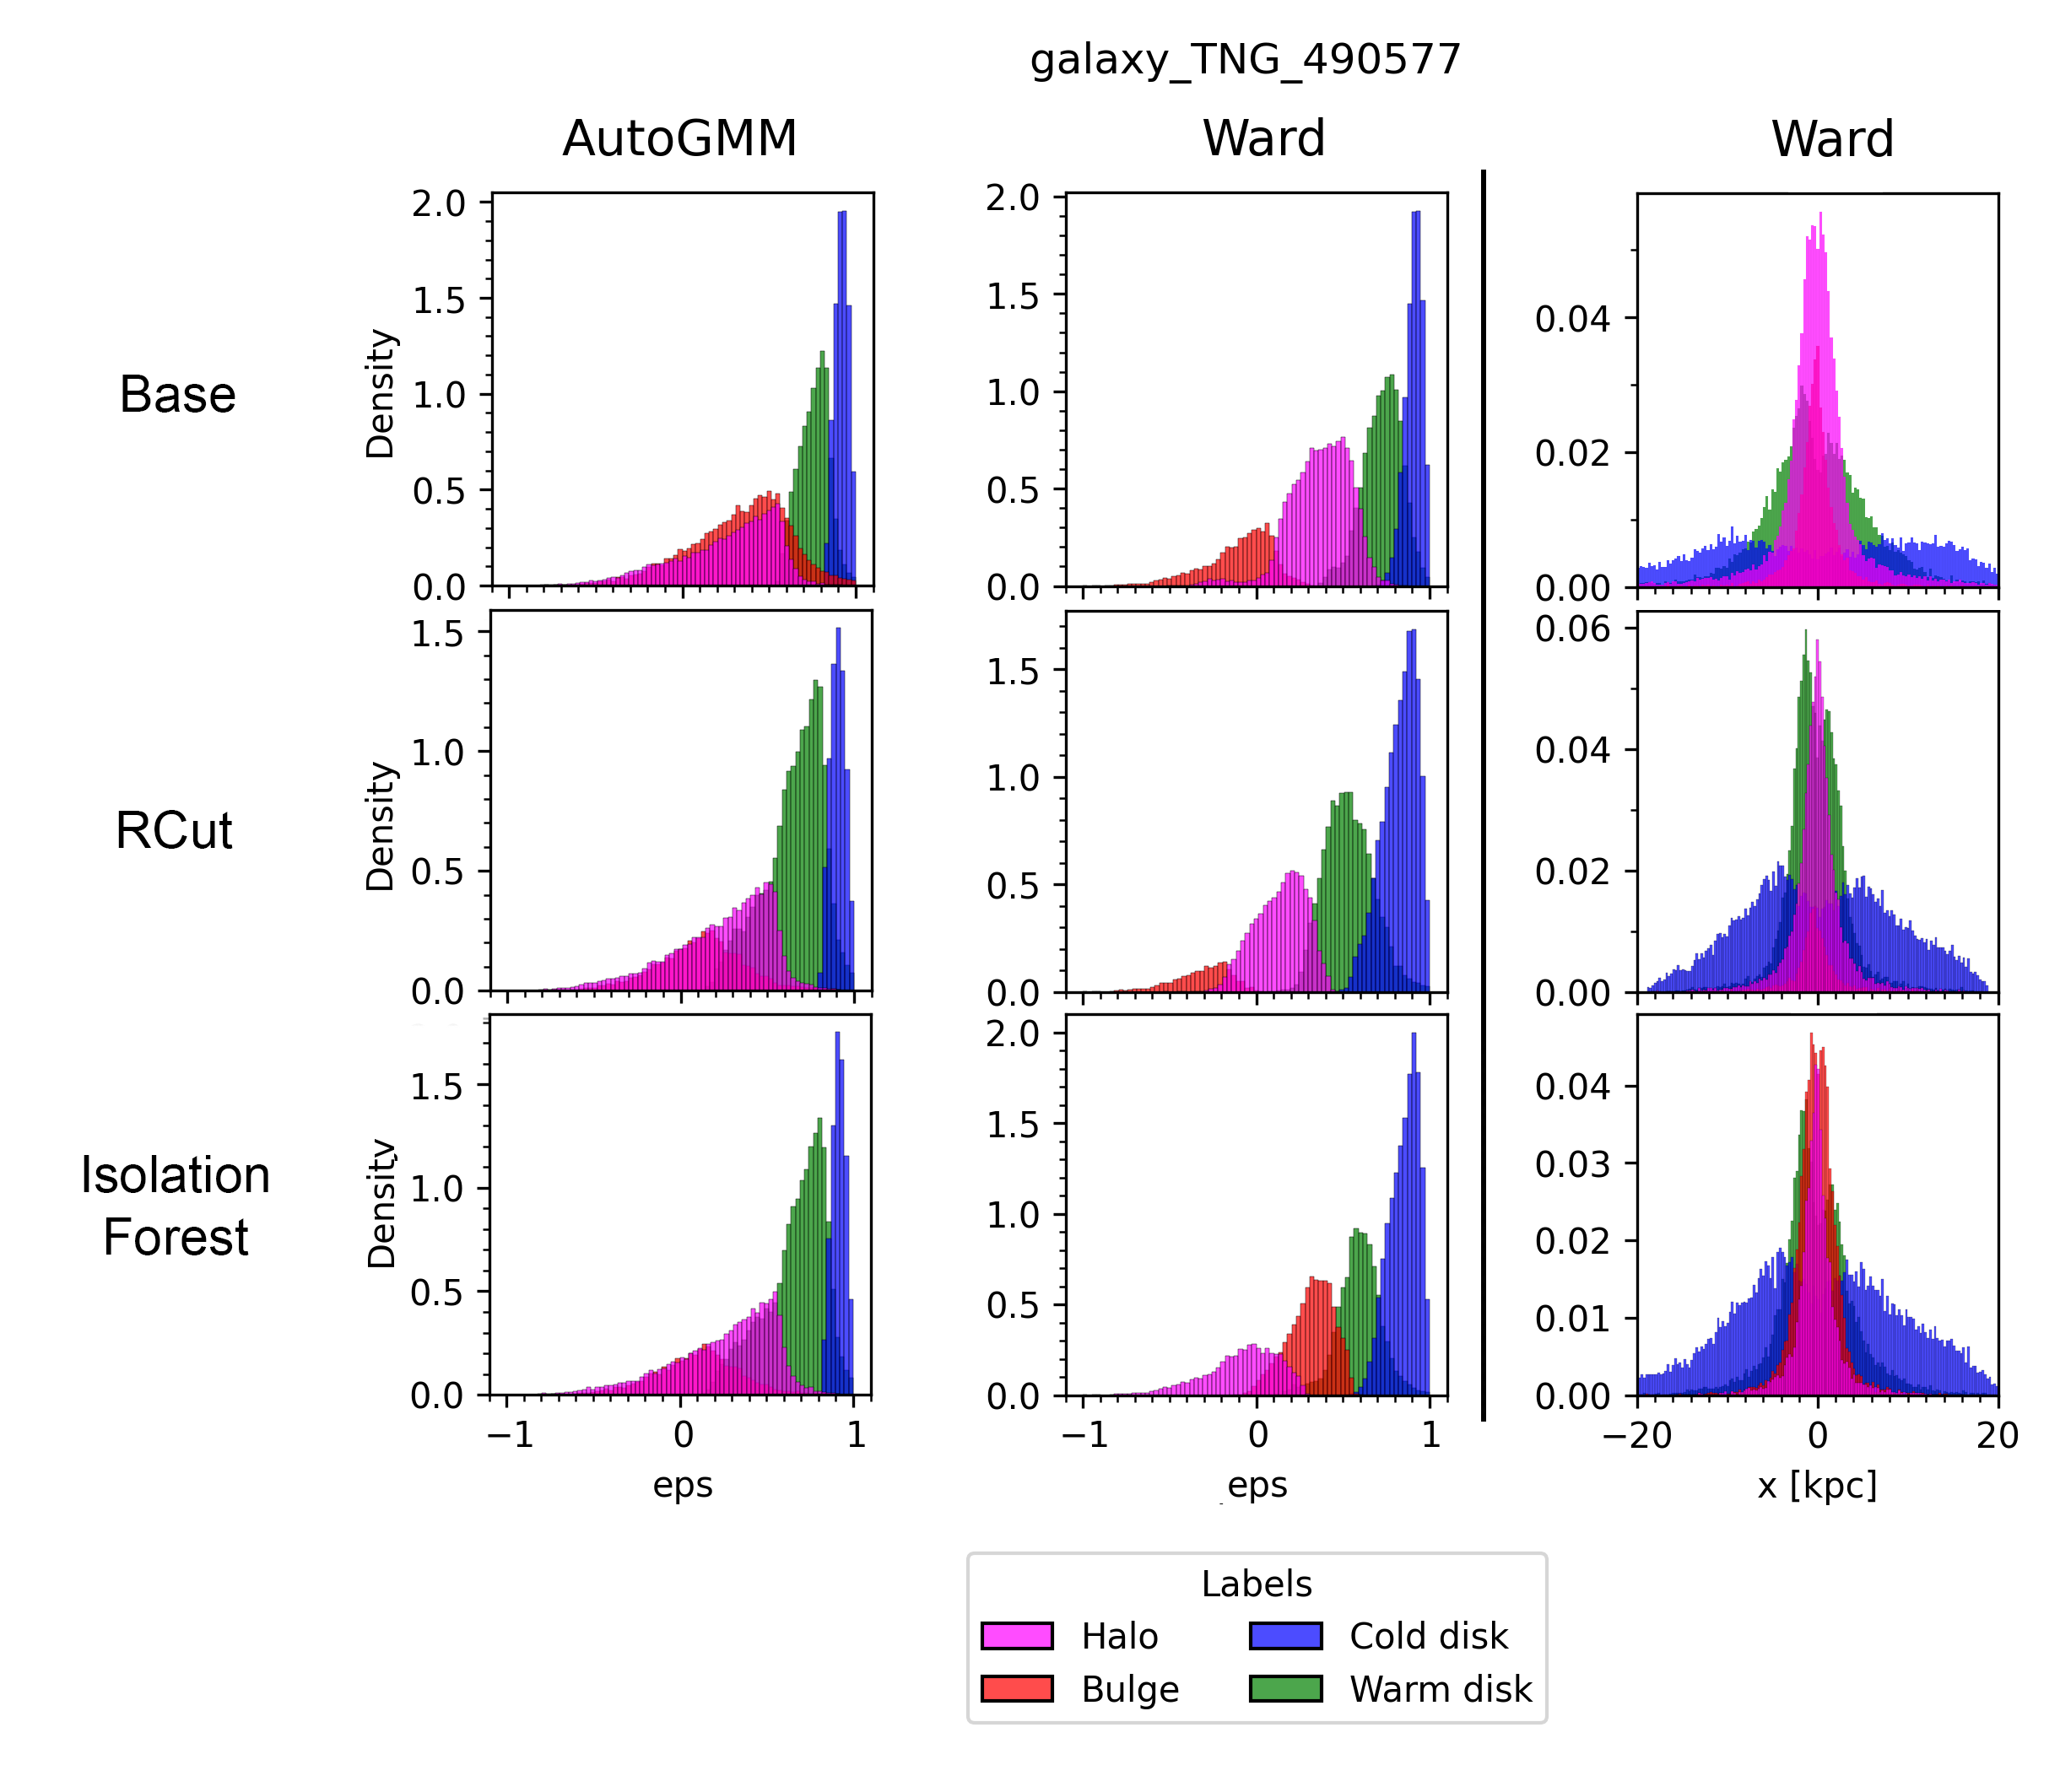
\includegraphics[width=9cm]{clustering jerarquico/figures/AGMM - galaxy_TNG_490577 - complete.png}
\end{center}

\note{
%- heuristica para asignar labels: maximiza el promedio pesado de los valores de Recall de cada conjunto encontrado de entre todas sus posibles permutaciones\\
%- aunque pareciera que hemos etiquetado de forma errónea al Halo y el Bulge en \gls{IF}, el método detallado nos provee una base sólida para razonar sobre los resultados. \\
- en el apendice tenemos mas ejemplos, pero dadas las galaxias cuya cardinalidad de componentes no vario al remover analisis (menos de la mitad de nuestro adataset), \textbf{no podemos concluir} tampoco si hacerlo nos da mejores o peores resultados.
}

\end{frame}

\iflong
\begin{frame}
\frametitle{AGMM: Eliminación de outliers}
\begin{center}
    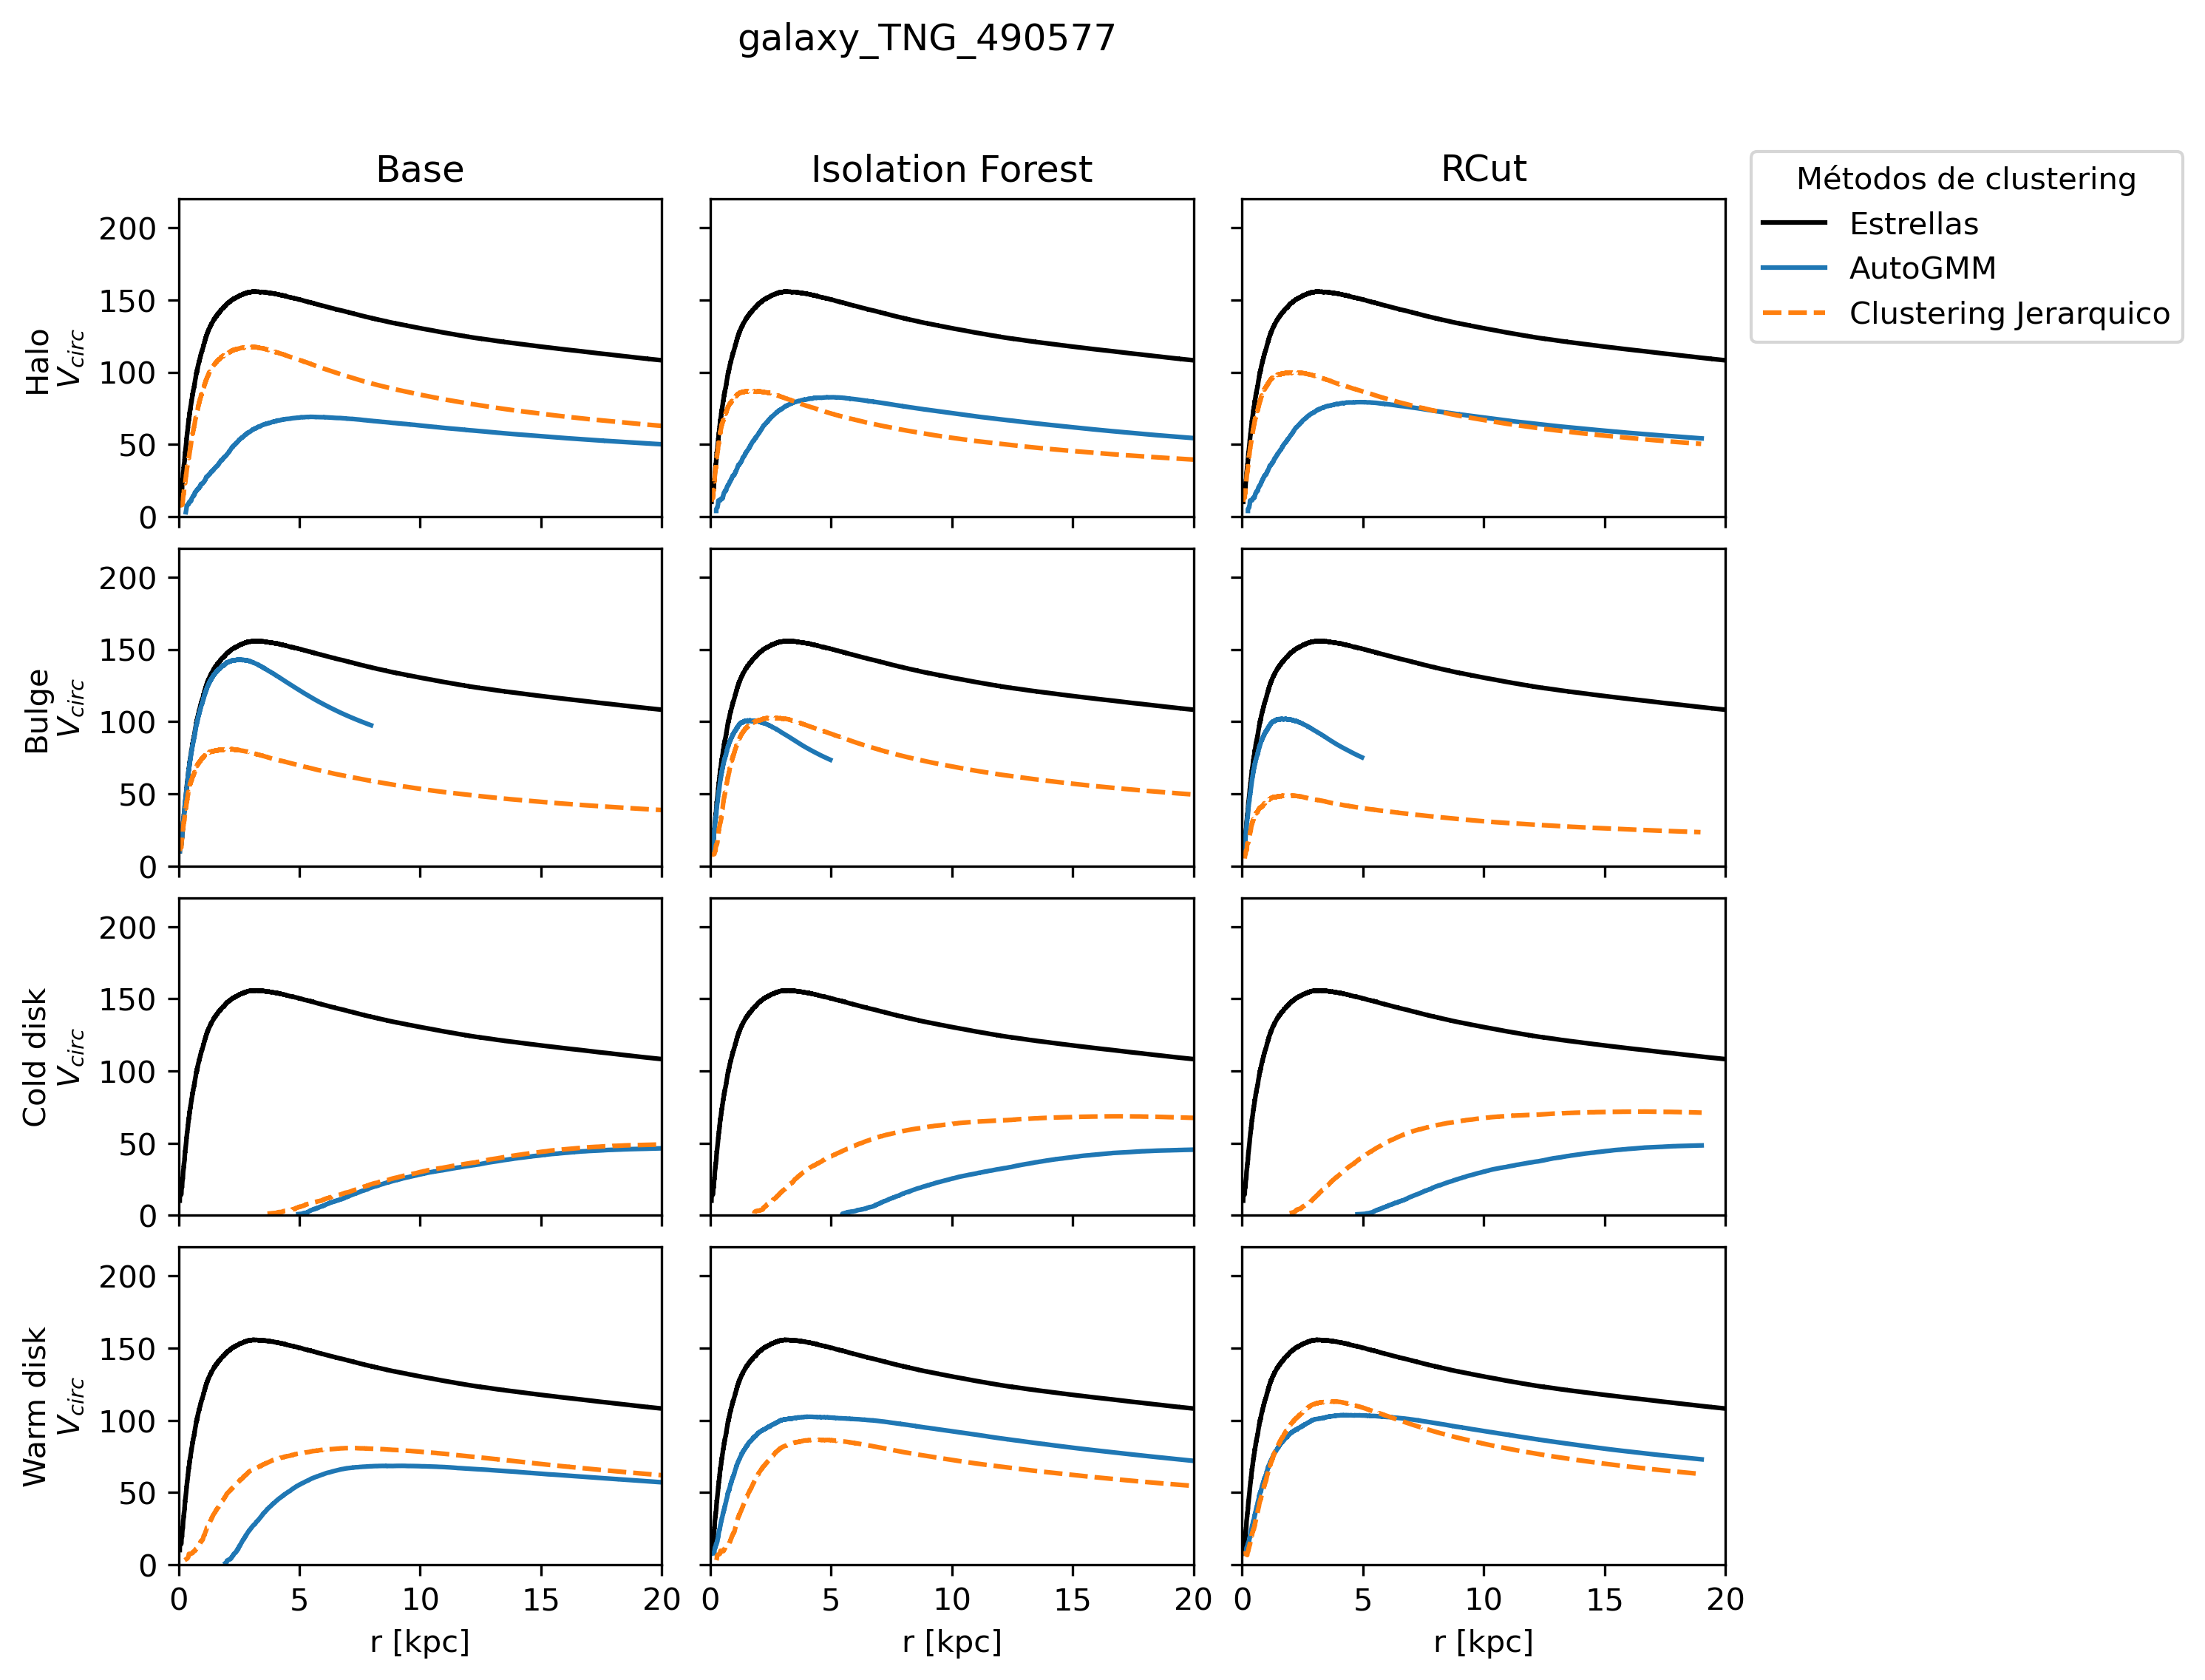
\includegraphics[width=10cm]{clustering jerarquico/figures/galaxy_TNG_490577 - AutoGMM - circ_velocity.png}
\end{center}

\note{
otro ejemplo
}

\end{frame}
\endif



